\chapter{数学知识总结}

%------------------------------------------------------------------------------
%                                Matrix Definations
%------------------------------------------------------------------------------
\section{各类矩阵定义}
%转置矩阵
\begin{definition}{\hypertarget{transpose}{转置矩阵}}{int}
\label{def:transpose}
把矩阵$A$的行换乘同序数的列得到一个新矩阵,就叫做$A$的转置矩阵,记作$A^{T}$。例如矩阵
\begin{align}
A = 
\begin{bmatrix}
1 & 2 & 0 \\
3 & -1 & 1
\end{bmatrix}
\end{align}
的转置矩阵为
\begin{align}
A^{T} = 
\begin{bmatrix}
1 & 3 \\
2 & -1 \\
0 & 1
\end{bmatrix}
\end{align}
\end{definition}

%对称矩阵
\begin{definition}{\hypertarget{symmetric}{对称矩阵}}{int}
\label{def:symmetric}
设$A$为$n$阶方阵,如果满足$A^T=A$,即:
\begin{align}
a_{ij} = a_{ji}  (i,j=1, 2, ..., n)
\end{align}
那么$A$称为对称矩阵,简称为对称阵。对称阵的特点是:它的元素以对角线为对称轴对应相等。
\end{definition}

%复共轭矩阵
\begin{definition}{\hypertarget{ctranspose}{复共轭矩阵}}{int}
\label{def:ctranspose}
设$A\in{C^{m\times{n}}}$,用$\bar{A}$表示以$A$的元素的共轭复数为元素组成的矩阵,命:
\begin{align}
A^{H} = (\bar{A})^{T}
\end{align}
则称$A^{H}$为$A$的复共轭转置矩阵。
\end{definition}

%Hermitian矩阵
\begin{definition}{\hypertarget{hermitian}{Hermitian矩阵}}{int}
\label{def:hermitian}
设$A\in{R^{n\times{n}}}$,若$A^{H}=A$,则称$A$为Hermitian矩阵。若$A^{H}=-A$,则称$A$为反Hermitian矩阵。
\end{definition}

%正交矩阵
\begin{definition}{\hypertarget{orthogonal}{正交矩阵}}{int}
\label{def:orthogonal}
如果$n$阶矩阵$A$满足
\begin{align}
A^{T}A=E
\end{align}
即:
\begin{align}
A^{T}=A^{-1}
\end{align}
则称$A$为正交矩阵,简称正交阵。
\end{definition}

%酉矩阵
\begin{definition}{\hypertarget{unitary}{酉矩阵}}{int}
\label{def:unitary}
如果$n$阶复矩阵$A$满足
\begin{align}
A^{H}A=AA^{H}=E
\end{align}
则称$A$为酉矩阵,记作$A\in{U^{n\times{n}}}$。
\end{definition}

%奇异矩阵
\begin{definition}{\hypertarget{singular}{奇异矩阵}}{int}
\label{def:singular}
当$|A|=0$时,$A$称为奇异矩阵,否则称为非奇异矩阵。$A$是可逆矩阵的充分必要条件是$|A|\neq{0}$,即可逆矩阵就是非奇异矩阵。
\end{definition}

%正规矩阵
\begin{definition}{\hypertarget{formal}{正规矩阵}}{int}
\label{def:formal}
设$A\in{C^{n\times{n}}}$,若:
\begin{align}
A^{H}A=AA^{H}
\end{align}
则称$A$为正规矩阵,$A\in{R^{n\times{n}}}$,显然有$A^{H}=A^{T}$,上式就变成了:
\begin{align}
A^{T}A=AA^{T}
\end{align}
则称$A$为实正规矩阵。
\end{definition}

%幂等矩阵
\begin{definition}{\hypertarget{power}{幂等矩阵}}{int}
\label{def:power}
设$A\in{C^{n\times{n}}}$,若:
\begin{align}
A^{2}=A
\end{align}
则称$A$是幂等矩阵。
\end{definition}

%正定矩阵
\begin{definition}{\hypertarget{positive}{正定矩阵}}{int}
\label{def:positive}
设$A\in{C^{n\times{n}}}$,若A的所有特征值均为正数,则称$A$为正定矩阵;若$A$的特征值均为非负数,则称$A$为版正定矩阵。

判断一个矩阵为正定矩阵的充要条件有:
\begin{enumerate}
\item $A$的所有特征值$\lambda_{i}$均为正数;
\item $x^{T}Ax \ge 0$对所有非零向量$x$都成立;
\item 存在秩满矩阵$R$,使得$A=R^{T}R$。
\end{enumerate}
\end{definition}

%Jacobi矩阵
\begin{definition}{\hypertarget{power}{Jacobi矩阵}}{int}
\label{def:jacobi}
假设某函数从$f:R^{n}\rightarrow R^{m}$,从$x\in{R^{n}}$映射到向量$f(x)\in{R^{m}}$,其Jacobi矩阵的维度是$m\times{n}$,如下所示:
\begin{align}
H = 
\begin{bmatrix}
\frac{\partial f}{\partial x_{1}} & \frac{\partial f}{\partial x_{1}} & \cdots & \frac{\partial f}{\partial x_{n}} 
\end{bmatrix}
 =
\begin{bmatrix}
\frac{\partial f_{1}}{\partial x_{1}}  & \frac{\partial f_{1}}{\partial x_{2}} & \cdots & \frac{\partial f_{1}}{\partial x_{n}} \\
\frac{\partial f_{2}}{\partial x_{1}}  & \frac{\partial f_{2}}{\partial x_{2}} & \cdots & \frac{\partial f_{2}}{\partial x_{n}} \\
\vdots        & \vdots        & \ddots    & \vdots \\
\frac{\partial f_{m}}{\partial x_{1}}  & \frac{\partial f_{m}}{\partial x_{2}} & \cdots & \frac{\partial f_{m}}{\partial x_{n}} \\
\end{bmatrix}
\end{align}
\end{definition}

%Hessian矩阵
\begin{definition}{\hypertarget{power}{Hessian矩阵}}{int}
\label{def:hessian}
若实值函数$f(x_1, x_2, ..., x_n)$的所有二阶偏导都存在并在定义域内连续,那么函数$f$的Hessian矩阵为:
\begin{align}
H = 
\begin{bmatrix}
\frac{\partial^{2}f}{\partial x_{1}^{2}}  & \frac{\partial^{2}f}{\partial x_{1}x_{2}} & \cdots & \frac{\partial^{2}f}{\partial x_{1}x_{n}} \\
\frac{\partial^{2}f}{\partial x_{2}x_{1}} & \frac{\partial^{2}f}{\partial x_{2}^{2}}  & \cdots & \frac{\partial^{2}f}{\partial x_{2}x_{n}} \\
\vdots        & \vdots        & \ddots    & \vdots \\
\frac{\partial^{2}f}{\partial x_{n}x_{1}} & \frac{\partial^{2}f}{\partial x_{n}x_{2}} & \cdots & \frac{\partial^{2}f}{\partial x_{n}^{2}} \\
\end{bmatrix}
\end{align}
根据:
\begin{align}
\frac{\partial^{2}f}{\partial x_{1}x_{2}}  = \frac{\partial^{2}f}{\partial x_{2}x_{1}} 
\end{align}
可知Hessian矩阵为对称阵。
\end{definition}
%------------------------------------------------------------------------------
%                                         瑞利商
%------------------------------------------------------------------------------
\section{瑞利商}
\label{sec:rayleigh-quotient}
对于一个\hyperlink{hermitian}{Hermitian矩阵}$M$及非零向量$x$,\href{https://en.wikipedia.org/wiki/Rayleigh_quotient}{瑞利商}(Rayleigh quotient)的定义如公式\ref{eqn:ray1},其中$x^{H}$为$x$的共轭转置向量。
\begin{align}
\label{eqn:ray1}
R(M,x)=\frac{x^{H}Mx}{x^{H}x}
\end{align}

若$M$和$x$中元素均为实数,瑞利商可以写成公式\ref{eqn:ray2}。
\begin{align}
\label{eqn:ray2}
R(M,x)=\frac{x^{T}Mx}{x^{T}x}
\end{align}

设M的特征值与特征向量分别为$\lambda_1, ..., \lambda_n$和$v_1, .., v_n$,且满足 $\lambda_{\min}=\lambda_1\leq{\lambda_2}\leq{...}\leq{\lambda_n}=\lambda_{\max}$,那么在M已知的情况下有:
\begin{align}
\label{eqn:conc-ray}
\begin{split}
cR(M,x) &= \lambda_{n} \\
\mathop{\min}_{x}R(M,x) &= \lambda_{1}
\end{split}
\end{align}

以下为证明公式\ref{eqn:conc-ray}的过程:

由于$M$是Hermitian矩阵,存在一个酉矩阵$U$,满足公式\ref{eqn:unity-matrix}。
\begin{align}
\label{eqn:unity-matrix}
M=UAU^{T}
\end{align}
其中$A=diag\{\lambda_1, ..., \lambda_n\}$。

因此公式\ref{eqn:ray2}可以转换如下:
\begin{align}
\begin{split}
R(M,x) &= \frac{x^{T}UAU^{T}x}{x^{T}x} \\
       &= \frac{(U^{T}x)^{T}A(U^{T}x)}{x^{T}x}  
\end{split}
\end{align}

设$P=U^{T}x$,则:
\begin{align}
\label{eqn:trans1}
\begin{split}
R(M,x) &= \frac{P^{T}AP}{x^{T}x} \\
       &= \frac{\sum_{i=1}^{n}\lambda_{i}|P_i|^{2}}{\sum_{i=1}^{n}|x_i|^{2}}
\end{split}
\end{align}

根据特征值的大小关系,我们可以得到不等式\ref{eqn:feature-unequal}。
\begin{align}
\label{eqn:feature-unequal}
\lambda_{1}\sum_{i=1}^{n}|P_i|^{2} \leq \sum_{i=1}^{n}\lambda_{i}|P_i|^{2} \leq \lambda_{n}\sum_{i=1}^{n}|P_i|^{2}
\end{align}

所以公式\ref{eqn:trans1}的范围如下:
\begin{align}
\label{eqn:trans0}
\lambda_{1}\frac{\sum_{i=1}^{n}|P_i|^{2}}{\sum_{i=1}^{n}|x_i|^{2}} \leq R(M,x) \leq \lambda_{n}\frac{\sum_{i=1}^{n}|P_i|^{2}}{\sum_{i=1}^{n}|x_i|^{2}} 
\end{align}

设$U$第$i$行第$j$列的元素为$u_{ij}$,则$U^{T}$第$i$行第$j$列的元素为$u_{ji}$,由$P=U^{T}x$和$P^{T}=x^{T}U$可得:
\begin{align}
\begin{split}
p_i &= \sum_{i=1}^{n} u_{ji}x_j \\
p_{i}^{T} &= \sum_{j=1}^{n} x_{i}u_{ij}
\end{split}
\end{align}

则:

\begin{align}
|p_i|^{2} = p_{i}^{T}p_i = \sum_{j=1}^{n} \sum_{k=1}^{n} x_j u_{ij} u_{ki} x_k
\end{align}

于是:
\begin{align}
\label{eqn:trans2}
\begin{split}
\sum_{i=1}^{n}|p_i|^{2} &= \sum_{i=1}^{n} p_{i}^{T}p_i \\
                        &= \sum_{i=1}^{n} \sum_{j=1}^{n} \sum_{k=1}^{n} x_j u_{ij} u_{ki} x_k \\
                        &= \sum_{j=1}^{n} \sum_{k=1}^{n} (\sum_{i=1}^{n} u_{ki} u_{ij}) x_j x_k 
\end{split}
\end{align}

因为$U$是酉矩阵,满足$U^{T}U=I$,所以:
\begin{align}
I_{jk} = \sum_{i=1}^{n} u_{ji} u_{ik}
\end{align}

其满足如下等式:
\begin{equation}
\label{eqn:trans3}
I_{jk}=\left\{
\begin{array}{rcl}
1 & & j = k\\
0 & & j \neq k
\end{array} \right
\end{equation}

结合\ref{eqn:trans2}和\ref{eqn:trans3}可得如下等式:
\begin{align}
\sum_{i=1}^{n}|p_i|^{2} = \sum_{i=1}^{n} |x_i|^2
\end{align}

代入公式\ref{eqn:trans0}可得:
\begin{align}
\label{eqn:trans4}
\lambda_{1} \leq R(M,x) \leq \lambda_{n} 
\end{align}
且:
\begin{equation}
\label{eqn:trans5}
R(M,x)=\left\{
\begin{array}{rcl}
\lambda_{1} & & x = v_1\\
\lambda_{n} & & x = v_n
\end{array} \right
\end{equation}

如果用$x^{'}=cx$代入公式\ref{eqn:ray2}有:
\begin{align}
\begin{split}
R(M,x^{'})  &=\frac{x^{'}^{T}Mx^{'}}{x^{'}^{T}x^{'}}  \\
            &=\frac{c^{2}x^{T}Mx}{c^{2}x^{T}x}  \\
            &=\frac{x^{T}Mx}{x^{T}x} 
\end{split}
\end{align}

由此可以看出来对$x$进行缩放不影响瑞利商的值,即:
\begin{align}
R(M,cx) = R(M,x) 
\end{align}

因此我们可以限定$x^Tx=1$,那么公式\ref{eqn:ray2}可以简化为:
\begin{align}
R(M,x) = x^{T}Mx
\end{align}

那么$R(M,x)$的极值就可以转换成约束条件下的拉格朗日乘法,如公式\ref{eqn:lage}。
\begin{align}
\label{eqn:lage}
L(x, \lambda) = x^{T}Mx - \lambda(x^{T}x-1)
\end{align}

对$x$求导并置为0可得:
\begin{align}
\nabla{L(x, \lambda)} = Mx - \lambda{x} = 0
\end{align}
即$M$的特征值能使得瑞利商取极值,且有:
\begin{align}
R(M,x) = \lambda
\end{align}

瑞利商可以推广至广义瑞利商(Generalized Rayleigh Quotient),其形式如公式\ref{eqn:GRQ}。
\begin{align}
\label{eqn:GRQ}
R(A,B,x) = \frac{x^{H}Ax}{x^{H}Bx}
\end{align}
其中$A$, $B$均为$n\times{n}$的Hermitian矩阵,且$B$为正定矩阵。

令$x=B^{-\frac{1}{2}}x^{'}$,广义瑞利商可以改写成:
\begin{align}
\label{eqn:GRQ}
\begin{split}
R(A,B,x) &= \frac{(B^{-\frac{1}{2}}x^{'})^{H}A(B^{-\frac{1}{2}}x^{'}))}{(B^{-\frac{1}{2}}x^{'})^{H}B(B^{-\frac{1}{2}}x^{'})} \\
         &= \frac{x^{'}^{H}(B^{-\frac{1}{2}})^{H}AB^{-\frac{1}{2}}x^{'}}{x^{'}^{H}(B^{-\frac{1}{2}})^{H}BB^{-\frac{1}{2}}x^{'}}  \\
         &= \frac{x^{'}^{H}(B^{-\frac{1}{2}})^{H}AB^{-\frac{1}{2}}x^{'}}{x^{'}^{H}x^{'}}
\end{split}
\end{align}

此时$R(A,B,x)$的最大特征值和最小特征值即为$(B^{-\frac{1}{2}})^{H}AB^{-\frac{1}{2}}$的最大和最小特征值。其实等价于当$M=(B^{-\frac{1}{2}})^{H}AB^{-\frac{1}{2}}$时的$R(M,x^{'})$,$x^{'}=B^{\frac{1}{2}}x$。

为简单起见,我们可以令$P=B^{-\frac{1}{2}}$,公式\ref{eqn:GRQ}可以写作:
\begin{align}
\label{eqn:GRQ1}
\begin{split}
R(A,B,x) &= \frac{x^{'}^{H}(B^{-\frac{1}{2}})^{H}AB^{-\frac{1}{2}}x^{'}}{x^{'}^{H}x^{'}} \\
         &= \frac{x^{'}^{H}P^{H}APx^{'}}{x^{'}^{H}x^{'}}  \\
         &= \frac{(Px^{'})^{H}APx^{'}}{x^{'}^{H}x^{'}}
\end{split}
\end{align}

类比上面提到的拉格朗日乘法,我们可以得到如下等式:
\begin{align}
\nabla{L(x, \lambda)} = P^{H}APx^{'} - \lambda{x^{'}} = 0
\end{align}

代入$x^{'}=P^{-1}x$有:
\begin{align}
\nabla{L(x, \lambda)} = P^{H}APP^{-1}x - \lambda{P^{-1}x} 
\end{align}

解得:
\begin{align}
PP^{H}Ax=\lambda{x} 
\end{align}

又因为$B^{-1}=PP^{H}$,所以最终求解特征值和特征向量可以依据:
\begin{align}
B^{-1}Ax=\lambda{x}
\end{align}

%------------------------------------------------------------------------------
%                                        EM算法
%------------------------------------------------------------------------------
\section{EM算法}
\label{sec:em}
本节来自于Andrew Ng的课堂讲义\upcite{em-alg}以及李航老师的《统计学习方法》\upcite{stat-lihang}。

\subsection{Jensen's Inequality}
首先介绍一下\href{https://en.wikipedia.org/wiki/Jensen\%27s_inequality}{Jensen不等式}。

定义$f$为实域的函数,若$f^{''}(x) \geq 0$,$x\in{R}$,则$f$为凸函数。若自变量$x$为向量,则当$f$关于$x$的Hessian矩阵为半正定矩阵,即$H \geq 0$时,$f$为凸函数;

如果对于所有的$x\in{R}$,有$f^{''}(x)>0$或对于所有的向量$x$,有$H>0$,$f$为严格意义上的凸函数。那么Jensen不等式定义定理\ref{thm:jensen-ineq}:
\begin{theorem}{Jsensen's Inequality}{jensen-ineq}
假定$f$是一个凸函数,$X$是一个随机变量,那么:
\begin{equation}
E[f(X)] \geq f(EX)
\end{equation}
\end{theorem}

且,如果$f$是严格凸函数,则当且仅当$X=E[X]$时定理\ref{thm:jensen-ineq}取等号。图\ref{fig:jesen-inequality}提供了一个理解Jensen不等式的例子。
\begin{figure}[h]
  \centering
  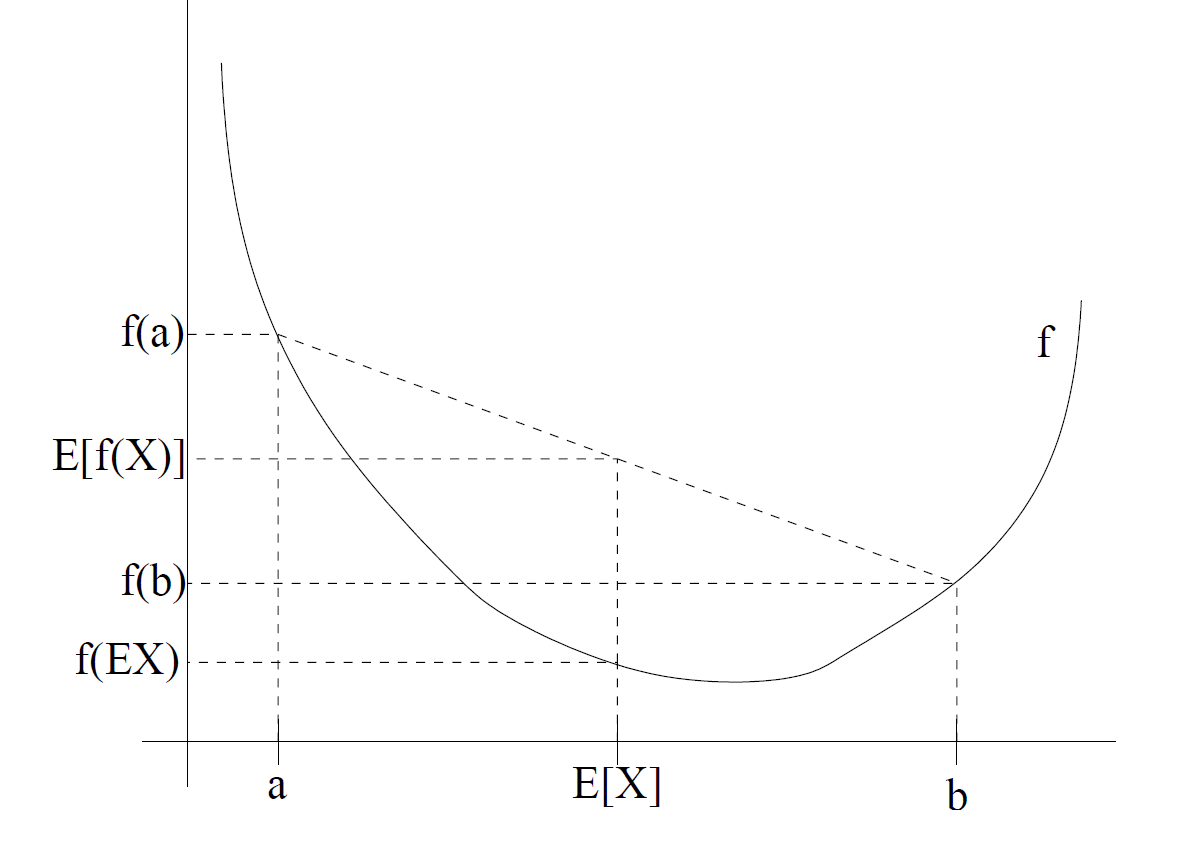
\includegraphics[width=0.55\textwidth]{jesen-inequality}
  \caption{Jensen's Inequality示例 \label{fig:jesen-inequality}}
\end{figure}

图中实线部分$f$是一个凸函数,随机变量$X$分别以$0.5$的概率取值$a$和$b$,因此随机变量$X$的期望为$a$和$b$的中间值,即:
\begin{align}
\label{eqn:exam-jsen}
  EX = \frac{a+b}{2}
\end{align}
期望对应的函数值为$f(EX)$,如图所示。而$E[f(X)]$等于:
\begin{align}
\label{eqn:exam-jsen1}
  E[f(X)] = \frac{f(a)+f(b)}{2}
\end{align}

从图上我们可以很明显的看出来二者的大小关系,又因为$X$是随机变量,当我们取$X=EX$的时候,函数的期望$E[f(x)]$和期望的函数$f(EX)$是相等的,所以有定理\ref{thm:jensen-ineq}。

\subsection{EM算法推导}
一般地,用$X$表示观测随机变量的数据,$Z$表示隐随机变量的数据,$X$和$Z$连在一起称为完全数据。观测数据$X$又称为不完全数据。假设给定观测数据$X$,其概率分布是$P(X|\theta)$,其中$\theta$是需要估计的参数,那么不完全数据$X$的似然函数是$P(X|\theta)$,对数似然函数是$L(\theta)=\log P(X|\theta)$;假设$X$和$Z$的联合概率分布是$P(X,Z|\theta)$,那么完全数据的对数似然函数是$L(\theta)=\log P(X,Z|\theta)$。

假设有$m$个相互独立的训练样本$\{x^{(1)},...,x^{(m)}\}$,我们需要估计这$m$个样本概率分布的参数。若隐变量为$z$,想要找到拟合模型$p(x,z)$的参数,其对数似然函数如公式\ref{eqn:em-likelihood}。
\begin{align}
\label{eqn:em-likelihood}
\begin{split}
  l(\theta) &= \sum_{i=1}^{m} \logp(x_{(i)}; \theta) \\
            &= \sum_{i=1}^{m} \log \sum_{z} p(x_{(i)}|z;\theta)p(x;\theta) \\
            &= \sum_{i=1}^{m} \log \sum_{z} p(x^{(i)}, z;\theta)
\end{splits}
\end{align}

由于隐变量$z$的存在,导致很难使用最大似然估计来得到参数$\theta$,在这种情况下,EM算法做的事情是给似然函数找个下界(E步),然后最大化这个下界(M步),如此反复迭代多次,最终收敛为止。

对于每一个样本$x^{(i)}$,我们定义$Q_{i}$为隐随机变量$z$的分布,其满足:
\begin{align}
\label{eqn:z-dis}
  \sum_{z} Q_{i}(z) = 1, \  Q_{i}(z) \geq 0
\end{align}
下面,我们来推导一下EM算法的精髓过程,见公式\ref{eqn:em-tuidao}。
\begin{align}
\label{eqn:em-tuidao}
\begin{split}
  \sum_{i=1}^{m} \logp(x_{(i)}; \theta) 
            &= \sum_{i=1}^{m} \log \sum_{z^{(i)}} p(x^{(i)}, z;\theta) \\
            &= \sum_{i=1}^{m} \log \sum_{z^{(i)}} Q_{i}(z^{(i)}) \frac{p(x^{(i)}, z;\theta)}{Q_{i}(z^{(i)})} \\
            &\geq \sum_{i=1}^{m} \sum_{z^{(i)}}  Q_{i}(z^{(i)}) \log \frac{p(x^{(i)}, z;\theta)}{Q_{i}(z^{(i)})}
\end{split}
\end{align}

公式\ref{eqn:em-tuidao}的最后一步是通过Jensen's Inequality得到的。我们分析下这个推导。

首先我们知道对数函数为凹函数,因为对数函数的二阶导$f^{''}(x)=-1/x^{2}<0$,其中$x\in{R^{+}}$。而
\begin{align}\nonumber
\label{eqn:em-expe}
\sum_{z^{(i)}} Q_{i}(z^{(i)}) \frac{p(x^{(i)}, z;\theta)}{Q_{i}(z^{(i)})}
\end{align}
是
\begin{align}\nonumber
\label{eqn:em-expe1}
\frac{p(x^{(i)}, z;\theta)}{Q_{i}(z^{(i)})}
\end{align}
关于服从分布$Q_{i}$的随机变量$z_{i}$期望。

由Jensen's Inequality可以得到公式\ref{eqn:em-jensen}:
\begin{align}
\label{eqn:em-jensen}
f\Bigg(E_{z^{(i)}\sim Q_{i}}\Big [\frac{p(x^{(i)}, z;\theta)}{Q_{i}(z^{(i)})}\Big ]\Bigg) \geq  E_{z^{(i)}\sim Q_{i}}\Bigg [f\Big(\frac{p(x^{(i)}, z;\theta)}{Q_{i}(z^{(i)})}\Big)\Bigg ]
\end{align}

其中下角标${z^{(i)}\sim Q_{i}}$表示这个期望是针对服从分布$Q_{i}$的随机变量$z^{(i)}$,根据公式\ref{eqn:em-jensen}就可以推出\ref{eqn:em-tuidao}的最后一步。

ok,关于公式\ref{eqn:em-jensen}多说两句,这里面其实用到的公式就是Jensen不等式,但是这个式子和前面我们提到的定理\ref{thm:jensen-ineq}中的区别在于$E[f(X)] \geq f(EX)$中的$X$同样是个函数,其等于:
\begin{align}\nonumber
\label{eqn:em-expe1}
\frac{p(x^{(i)}, z;\theta)}{Q_{i}(z^{(i)})}
\end{align}

以上公式\ref{eqn:em-tuidao}给$l{\theta}$提供了一个下界,我们不断地最大化这个下界,就可以不断地增加$l(\theta)$,说明每一次迭代模型都能找到拟合的更好的参数。

好的,下一个问题是,我们如何最大化这个下界呢?假设$t$轮迭代后的参数为$\theta^{(t)}$,我们希望通过这个$\theta^{(t)}$来得到$Q_{i}(z^{(i)})$,即隐变量的分布。而$t$轮迭代的时候一定是满足下界最大化的,而最大化很明显就是变不等号为等号的临界部分,即定理\ref{thm:jensen-ineq}中等号成立的条件。所以第$t$轮得到的$\theta^{(t)}$必然满足公式\ref{eqn:theta-1}。
\begin{align}
\label{eqn:theta-1}
E_{z^{(i)}\sim Q_{i}}\Big [\frac{p(x^{(i)}, z;\theta)}{Q_{i}(z^{(i)})}\Big ] = \frac{p(x^{(i)}, z;\theta)}{Q_{i}(z^{(i)})}
\end{align}
展开之后有:
\begin{align}
\label{eqn:theta-2}
\begin{split}
\sum_{z} Q_{i}(z^{(i)} \frac{p(x^{(i)}, z;\theta)}{Q_{i}(z^{(i)})}
    &= \sum_{z} p(x^{(i)}, z;\theta) \\
    &= \frac{p(x^{(i)}, z;\theta)}{Q_{i}(z^{(i)})}
\end{split}
\end{align}

所以我们有:
\begin{align}
\label{eqn:theta-2}
\begin{split}
  Q_{i}(z^{(i)}) &= \frac{p(x^{(i)}, z;\theta)}{\sum_{z} p(x^{(i)}, z;\theta)} \\
                 &= \frac{p(x^{(i)}, z;\theta)}{p(x^{(i)} ;\theta)} \\
                 &= p(z | x^{(i)};\theta)
\end{split}
\end{align}

上面的推导过程其实就是EM算法中的E步。

总结下EM算法步骤:
\begin{enumerate}
  \item E步:对于每一个样本,作:
    \begin{align}
    \label{eqn:estep}
      Q_{i} \coloneqq p(z | x^{(i)};\theta)
    \end{align}
  \item M步:
    \begin{align}
    \label{eqn:mstep}
      \theta \coloneqq \arg\mathop{\max}_{\theta} \sum_{i=1}^{m} \sum_{z^{(i)}}  Q_{i}(z^{(i)}) \log \frac{p(x^{(i)}, z;\theta)}{Q_{i}(z^{(i)})}
    \end{align}  
\end{enumerate}}

在用EM算法求模型参数的时候,首先定义模型的初始化参数,得到初始化参数之后,我们就可以得到隐随机变量$z$的分布,得到这个分布之后,我们再通过M步去算最大似然概率,得到新的参数,如此反复迭代,最终到EM算法收敛为止。

\subsection{EM算法收敛性证明}
如何证明EM算法最终一定会收敛呢?假设$\theta^{(t)}$和$\theta^{(t+1)}$为连续的两次迭代后的参数,我们只需要证明最大似然随着迭代次数是单调递增即可,即证明不等式\ref{eqn:em-conv}。
\begin{align}
\label{eqn:em-conv}
\theta^{(t+1)} \geq \theta^{(t)}
\end{align}

根据$t$轮迭代后的参数$\theta^{(t)}$,我们可以得到
\begin{align}\nonumber
\label{eqn:em-q}
Q_{i}^{(t)} = p(z | x^{(i)};\theta^{(t)})
\end{align}

那么$t$步的似然度为(此时公式\ref{eqn:em-tuidao}的最后一步取等号):
\begin{align}\nonumber
\label{eqn:em-like}
l(\theta^{(t)}) = \sum_{i=1}^{m} \sum_{z^{(i)}}  Q_{i}^{(t)}(z^{(i)}) \log \frac{p(x^{(i)}, z;\theta^{(t)})}{Q_{i}^{(t)}(z^{(i)})}
\end{align}

参数$\theta^{(t+1)}$则是通过最大化上述公式得到的。因此我们有:
\begin{align}
l(\theta^{(t+1)}) &\geq  \sum_{i=1}^{m} \sum_{z^{(i)}}  Q_{i}^{(t)}(z^{(i)}) \log \frac{p(x^{(i)}, z;\theta^{(t+1)})}{Q_{i}^{(t)}(z^{(i)})} \label{eqn:em-1} \\
                  &\geq  \sum_{i=1}^{m} \sum_{z^{(i)}}  Q_{i}^{(t)}(z^{(i)}) \log \frac{p(x^{(i)}, z;\theta^{(t)})}{Q_{i}^{(t)}(z^{(i)})} \label{eqn:em-2} \\
                  &= l(\theta^{(t)})  \label{eqn:em-3}
\end{align}

不等式\ref{eqn:em-1}是由公式\ref{eqn:em-tuidao}推导出来的,其对于任意的$Q_{i}$和$\theta$都是成立的,自然对于$Q_{i}=Q_{i}^{(t)}$和$\theta=\theta^{(t)}$也成立。而不等式\ref{eqn:em-2}是通过EM算法中的M步得到的,因为:
\begin{align}
  \theta^{(t+1)} = \arg\mathop{\max}_{\theta} \sum_{i=1}^{m} \sum_{z^{(i)}}  Q_{i}^{(t)}(z^{(i)}) \log \frac{p(x^{(i)}, z;\theta)}{Q_{i}^{(t)}(z^{(i)})}
\end{align}  

公式\ref{eqn:em-3}即为Jensen不等式处于临界条件时的结果。

由此可以得知$l(\theta)$是随着迭代次数的增加单调递增的,即似然度是单调收敛的。因此EM算法的终止条件是似然度收敛,即似然度不会再增加了为止。但是实际情况中一般是看两个相邻的迭代过程似然度的差是否低于一个预设的值,如果低于该值,则停止迭代。

定义公式\ref{eqn:jesen-1}:
\begin{align}
\label{eqn:jesen-1}
  J(Q,\theta) = \sum_{i=1}^{m} \sum_{z^{(i)}}  Q_{i}(z^{(i)}) \log \frac{p(x^{(i)}, z;\theta)}{Q_{i}(z^{(i)})}
\end{align}

我们知道$l(\theta) \geq J(Q,\theta)$,我们也可以把EM算法看成一个坐标上升的过程,在E步的时候,相当于固定$\theta$求$Q$;在M步的时候,相当于固定了$Q$求$\theta$。

{\bf 题外话:}这个固定一个变量,最大化另外一个变量,通过另外一个变量求这个变量这个思想感觉跟GAN很类似啊……GAN里面也是这样的,先固定生成器,优化判别器;然后固定判别器,优化生成器。有时间把这两个联系到一起来想想,还挺有意思的……
%------------------------------------------------------------------------------
%                                        GMM
%------------------------------------------------------------------------------
\section{混合高斯分布}

%方差
\begin{definition}{方差}{int}
方差用于描述数据的离散或波动程度。假定变量为$X$,均值为$\bar{X}$,$N$为总体样本数,方差计算公式如下:
\begin{align}
var(X) = \frac{\sum_{i=1}^{N}(X_i-\bar{X})^{2}}{N-1}
\end{align}
\end{definition}

%协方差
\begin{definition}{协方差}{int}
协方差表示了变量线性相关的方向,取值范围是$[-\infty, \infty]$,一般来说协方差为正值,说明一个变量变大另一个变量也变大;取负值说明一个变量变大另一个变量变小,取0说明两个变量没有相关关系.
\begin{align}
cov(X) = \frac{\sum_{i=1}^{N}(X_i-\bar{X})^{2}(Y_i-\bar{Y})^{2}}{N-1}
\end{align}
\end{definition}

%相关系数
\begin{definition}{相关系数}{int}
协方差可反映两个变量之间的相互关系及相关方向,但无法表达其相关的程度,皮尔逊相关系数不仅表示线性相关的方向,还表示线性相关的程度,取值$[-1,1]$,也就是说,相关系数为正值,说明一个变量变大另一个变量也变大;取负值说明一个变量变大另一个变量变小,取0说明两个变量没有相关关系,同时,相关系数的绝对值越接近1,线性关系越显著。
\begin{align}
\rho_{XY} = \frac{cov(X, Y)}{\sqrt{DX}\sqrt{DY}}
\end{align}
\end{definition}

%协方差矩阵
\begin{definition}{协方差矩阵}{int}
 当$X\in{R^{n}$为高维数据时,协方差矩阵可以很好的反映数据的性质,在协方差矩阵中,对角线元素反映了数据在各个维度上的离散程度,协方差矩阵为对角阵,非对角线元素反映了数据各个维度的相关性,其形式如下:
\begin{align}
\Sigma = 
\begin{bmatrix}
cov(x_1, x_1) & cov(x_1, x_2) & \cdots & cov(x_1, x_n) \\
cov(x_2, x_1) & cov(x_2, x_2) & \cdots & cov(x_2, x_n) \\
\vdots        & \vdots        & \ddots    & \vdots \\
cov(x_n, x_1) & cov(x_n, x_2) & \cdots & cov(x_n, x_n) 
\end{bmatrix}
\end{align}
\end{definition}

单变量高斯分布公式如\ref{eqn:gaussian},其中$\mu$和$\sigma^{2}$分别为均值和方差。
\begin{align}
\label{eqn:gaussian}
\mathcal{N}(x; \mu, \sigma) = \frac{1}{\sqrt{2\pi}\sigma}\exp{\{-\frac{(x-\mu)^{2}}{2\sigma^{2}}\}}
\end{align}

多变量高斯分布公式如\ref{eqn:mgaussian},其中$\mu$和$\Sigma$分别为均值和协方差矩阵。
\begin{align}
\label{eqn:mgaussian}
\mathcal{N}(x; \mu, \Sigma) = \frac{1}{(2\pi)^{-\frac{n}{2}}|\Sigma|^{\frac{1}{2}}}\exp{\{-\frac{1}{2}(x-\mu)^{T}\Sigma^{-1}(x-\mu)\}}
\end{align}

混合高斯模型(Gaussian Mixture Model)表示的是多个高斯分布叠加在一起的分布,其公式如\ref{eqn:GMM},其中$K$为高斯分量的个数,$\pi_{k}$为各个分量的权重,其满足$0 \leq \pi_{k} \leq 1$,且$\sum_{k=1}^{K}\pi_{k}=1$。$p(x)$表示的是多个高斯分量加权后的分布。
\begin{align}
\label{eqn:GMM}
p(x) = \sum_{k=1}^{K}\pi_{k}\mathcal{N}(x; \mu_{k}, \Sigma_{k})
\end{align}

那么给定一堆训练数据,我们如何根据这些数据来得到GMM的参数呢?

假设训练集$\{x^{(1)},...,x^{(m)}\}$,由于估计GMM的算法为无监督学习算法,因此这些数据都是没有标签的。我们用一个联合分布模型来对这些数据进行建模,即:
\begin{align}
p(x^{(i)}, z^{(i)})=p(x^{(i)}|z^{(i)})p(z^{(i)})
\end{align}
其中,$z^{i}\sim{Multinomial(\phi)}$,$s_{j} \geq 0$,且$\sum_{j=1}^{k} \phi_{j}=1$,$\phi_{j}$表示的是$p(z^{(i)}=j)$,此外$p(x^{(i)}|z^{(i)}=j)\sim{\mathcal{N}(\mu_j,\Sigma_j)}$。$k$表示的是$z^{(i)}$所能取的值的个数。

我们选取的模型假设每个$x^{(i)}$都由随机选取的$z^{(i)}$生成,$z^{(i)}\in\{1,...,k\}$。我们可以理解成GMM模型有$k$个高斯分量,$z$就是表征每个分量权重的随机变量,因此$z$就是隐变量。$p(z^{(i)})=\phi_{j}$就是$x^{(i)}$这个数据来源于分量$j$的概率。

综上,GMM模型的参数为$\mu,\Sigma,\phi$。现在的问题就是如何求解这些参数。我们可以得到似然函数如公式\ref{eqn:gmm-likelihood}。
\begin{align}
\label{eqn:gmm-likelihood}
\begin{split}
  l(\mu,\Sigma,\phi) 
      &= \sum_{i=1}^{m} \log p(x^{(i)};\mu,\Sigma,\phi) \\ 
      &= \sum_{i=1}^{m} \log \sum_{z_{(i)}=1}^{k} p(x^{(i)}|z^{(i)};\mu,\Sigma)p(z^{(i)};\phi)
\end{split}
\end{align}

如果我们直接对这个似然函数进行求导,由于隐变量的存在,我们无法得到关于参数的确切解。那么既然问题出在隐变量上,如果我们已经知道了每一个$x^{(i)}$所属的分量,公式\ref{eqn:gmm-likelihood}就可以写成公式\ref{eqn:gmm-likelihood1},需注意此时隐变量的分布我们还是不知道,我们只知道训练集中的样本分别属于哪一个高斯分量。
\begin{align}
\label{eqn:gmm-likelihood1}
\begin{split}
  l(\mu,\Sigma,\phi) 
        &= \sum_{i=1}^{m} \log p(x^{(i)}|z^{(i)};\mu,\Sigma)p(z^{(i)};\phi) \\
        &= \sum_{i=1}^{m} \Big[\log p(x^{(i)}|z^{(i)};\mu,\Sigma) + \log p(z^{(i)};\phi) \Big]
\end{split}
\end{align}

此时用最大似然概率求解的办法就可以得到这些参数,我们写细一点,求解一下看看。

首先,求解$\phi_j$,在此之前,我们可以看出$l$中与$\phi$相关的项为:
\begin{align}\nonumber
  \sum_{i=1}^{m} \log p(z^{(i)};\phi) 
\end{align}
我们知道$\phi$是服从多项式分布的,$\phi$受限于$\sum_{j=1}^{k} \phi_{j}=1$,因此关于$\phi$的求解我们需要构建一个拉格朗日函数如下:
\begin{align}\nonumber
      \mathcal{L}(\phi) = \sum_{i=1}^{m} \log p(z^{(i)};\phi) + \beta(\sum_{j=1}^{k} \phi_{j}-1)
\end{align}

因此关于求解$\phi$的步骤如公式\ref{eqn:gmm-phi1}:
\begin{align}
\label{eqn:gmm-phi1}
\begin{split}
  \frac{\partial \mathcal{L}(\phi)}{\partial \phi_j}
  &=\frac{\partial \sum_{i=1}^{m} \log p(z^{(i)};\phi) + \beta(\sum_{j=1}^{k} \phi_{j}-1)}{\partial \phi_j} \\
  &= \sum_{i=1}^{m} \frac{\partial \log p(z^{(i)};\phi)}{\partial \phi_j} \\
\end{split}
\end{align}

因为不一定每个$x^{(i)}$都有$j$分量产生,我们定义$1\{z^{(i)}=j\}$如下,也就是说第$i$个样本由第$j$个样本产生的时候,我们取为1。
\begin{equation}
1\{z^{(i)}=j\}=\left\{
\begin{array}{rcl}
1& & if \  z^{(i)}=j\\
0 & & otherwise\\
\end{array} \right.
\end{equation}

公式\ref{eqn:gmm-phi1}可以写成公式\ref{eqn:gmm-phi2}:
\begin{align}
\label{eqn:gmm-phi2}
\begin{split}
  \frac{\partial \mathcal{L}(\phi)}{\partial \phi_j}
  &=\frac{\partial \sum_{i=1}^{m} \log p(z^{(i)};\phi) + \beta(\sum_{j=1}^{k} \phi_{j}-1)}{\partial \phi_j} \\
  &= \sum_{i=1}^{m} 1\{z^{(i)}=j\} \frac{\partial \log \phi_j + \beta{\phi_{j}}}{\partial \phi_j} \\
  &= \sum_{i=1}^{m} 1\{z^{(i)}=j\} \Big[ \frac{1}{\phi_j} + \beta \Big]\\
\end{split}
\end{align}

令公式\ref{eqn:gmm-phi2}为0,解得:
\begin{align}
  \phi_j = \frac{\sum_{i=1}^{m} 1\{z^{(i)}=j\}}{-\beta}
\end{align}

由此可知:$\phi_j \propto \sum_{i=1}^{m} 1\{z^{(i)}=j\}$,又因为$\sum_{j=1}^{k} \phi_{j}=1$,将$\phi_j$代入约束条件有:
\begin{align}
  \sum_{j=1}^{k} \phi_j = \frac{ \sum_{j=1}^{k} \sum_{i=1}^{m} 1\{z^{(i)}=j\}}{-\beta} =1
\end{align}
即
\begin{align}
  -\beta = \sum_{j=1}^{k} \sum_{i=1}^{m} 1\{z^{(i)}=j\}
\end{align}
也就是说$-\beta$等于属于各个高斯分量的训练样本的和,也就是$m$。至此,我们可以得到如下公式:
\begin{align}
  \phi_j = \frac{1}{m}\sum_{i=1}^{m} 1\{z^{(i)}=j\}
\end{align}

接着我们来求$\mu$,如公式\ref{eqn:gmm-mu}。
\begin{align}
\label{eqn:gmm-mu}
\begin{split}
  \frac{\partial l(\mu,\Sigma,\phi)}{\partial \mu_j}
  &=\frac{\partial \sum_{i=1}^{m} \Big[\log p(x^{(i)}|z^{(i)};\mu,\Sigma) + \log p(z^{(i)};\phi) \Big]}{\partial \mu_j} \\
  &= \frac{\partial \sum_{i=1}^{m}\log p(x^{(i)}|z^{(i)};\mu,\Sigma)}{\partial \mu_j} \\
  &= \frac{\partial \sum_{i=1}^{m} 1\{z^{(i)}=j\} \log p(x^{(i)}|z^{(i)};\mu,\Sigma)}{\partial \mu_j} \\
  &= \frac{\partial \sum_{i=1}^{m} 1\{z^{(i)}=j\} \log{\mathcal{N}(x^{(i)}; \mu_j, \Sigma_j)} }{\partial \mu_j} \\
  &= \frac{\partial \sum_{i=1}^{m} 1\{z^{(i)}=j\} \log \frac{1}{(2\pi)^{-\frac{n}{2}}|\Sigma_j|^{\frac{1}{2}}} \exp{\{-\frac{1}{2}(x^{(i)}-\mu_j)^{T}\Sigma_j^{-1}(x^{(i)}-\mu_j)\}} }{\partial \mu_j} \\
  &= \frac{\partial \sum_{i=1}^{m} 1\{z^{(i)}=j\} [-\frac{1}{2}(x^{(i)}-\mu_j)^{T}\Sigma_j^{-1}(x^{(i)}-\mu_j)]}{\partial \mu_j} \\
  &= \frac{\partial \sum_{i=1}^{m} 1\{z^{(i)}=j\} [-\frac{1}{2}({x^{(i)}}^{T}\Sigma_j^{-1}{x^{(i)}} - \mu_j^{T}\Sigma_j^{-1}x^{(i)} - {x^{(i)}}^{T}\Sigma_j^{-1}\mu_j + \mu_j^{T}\mu_j)]}{\partial \mu_j} \\
  &= \frac{\partial \sum_{i=1}^{m} 1\{z^{(i)}=j\} [-\frac{1}{2}(-\mu_j^{T}\Sigma_j^{-1}{x^{(i)}} - {x^{(i)}}^{T}\Sigma_j^{-1}\mu_j + \mu_j^{T}\mu_j)]}{\partial \mu_j} \\
  &= \sum_{i=1}^{m} 1\{z^{(i)}=j\}\Sigma_j^{-1} ( {x^{(i)}} - \mu_j) 
\end{split}
\end{align}

令公式\ref{eqn:gmm-mu}为零,则有:
\begin{align}
\label{eqn:gmm-mu1}
\sum_{i=1}^{m} 1\{z^{(i)}=j\}\Sigma_j^{-1} ({x^{(i)}} - \mu_j) = 0
\end{align}
解得:
\begin{align}
\label{eqn:gmm-mu2}
\mu_j = \frac{\sum_{i=1}^{m} 1\{z^{(i)}=j\} x^{(i)}}{\sum_{i=1}^{m} 1\{z^{(i)}=j\}}
\end{align}
最后,根据方差的定义,我们可以计算出方差的值,如公式\ref{eqn:gmm-sigma}
\begin{align}
\label{eqn:gmm-sigma}
\Sigma_j = \frac{\sum_{i=1}^{m} 1\{z^{(i)}=j\} (x^{(i)}-\mu_j)(x^{(i)}-\mu_j)^{T}}{\sum_{i=1}^{m} 1\{z^{(i)}=j\}}
\end{align}

上面我们算了一下在已知每个样本所属的高斯分量的情况下参数$\phi,\mu,\Sigma$的估计值。回到最初那个问题,训练数据是没有标签的,那么怎么估计参数?

只要知道了每一个训练样本所属的高斯分量,我们就可以通过最大似然估计求出参数。既然如此,我们可以先随机的将训练样本进行分配,初始化时,随机指定每一个训练样本所属的高斯分量,结合\ref{sec:em}中讲的EM算法,我们可以算出$\phi,\mu,\Sigma$,再用这个参数来更新每一个样本所属的高斯分量,因为在得到参数后,我们将训练样本$x^{(i)}$代入到GMM中,可以得到该样本分别属于每一个高斯分量的概率值,即求取$p(z^{(i)}=j|x^{(i)};\phi,\mu,\Sigma), j\in\{1,...K\}$。得到这些概率之后,我们认为每一个高斯分量以权重$p(z^{(i)}=j|x^{(i)};\phi,\mu,\Sigma)$生成了样本$x^{(i)}$,知道这些权重之后就可以继续更新参数,这样往往复复,不停的迭代,就会不停的朝着正确分类的方向走去,最终收敛即可。

下面介绍下GMM参数估计的EM算法:
\begin{enumerate}
  \item E步:对于$i,j$,作:
    \begin{align}
    \label{eqn:gmm-estep}
      w_j^{(i)} \coloneqq p(z^{(i)}=j | x^{(i)};\phi, \mu, \Sigma)
    \end{align}
  \item M步:
    \begin{align}
    \label{eqn:gmm-mstep}
      \phi_j &\coloneqq \frac{1}{m}\sum_{i=1}^{m} w_j^{(i)} \\
      \mu_j  &\coloneqq \frac{\sum_{i=1}^{m} w_j^{(i)} x^{(i)}}{\sum_{i=1}^{m} w_j^{(i)}}  \\
      \Sigma &\coloneqq \frac{\sum_{i=1}^{m} w_j^{(i)} (x^{(i)}-\mu_j)(x^{(i)}-\mu_j)^{T}}{\sum_{i=1}^{m} w_j^{(i)}}
    \end{align}  
\end{enumerate}}
%------------------------------------------------------------------------------
%                                      HMM
%------------------------------------------------------------------------------
\section{HMM相关知识点总结}
本节笔记来自于CS229课程中Daniel Ramage的Hidden Markov Models Fundamentals\upcite{hmm-cs229}。
\subsection{Markov Models}
给定状态集合$S=\{s_1, s_2, ..., s_{|S|}\}$,我们可以观测到沿着时间线的序列$\vec{z}\in S^{T}$。比方说一个天气系统$S=\{sun, cloud, rain\}$,其$|S|=3$。假设连续五天观察到的天气序列为$\{z_1=s_{sun}, z_2=s_{cloud}, z_3=s_{cloud}, z_4=s_{rain}, z_5=s_{cloud}\}$。

上述天气系统中观测到的状态序列是时间线上的随机过程,如果不作进一步假设的话,$t$时刻的状态$s_j$可能是任意变量的函数,不仅仅包括从时刻$1$到时刻$t-1$的状态,甚至还包括一些没有建模的变量,所以我们作出两个{\bf Markov Assumptions}使模型更可行:
\begin{enumerate}
  \item {\bf Limited Horizon Assumption}:假设$t$时刻的处于某个状态的概率只取决于$t-1$时刻的状态。本假设的直观感受是:$t-1$时刻的状态囊括了对过去时刻状态的总结,因而可以用于预测$t$时刻的输出。即:
    \begin{align}
      \label{eqn:lha}
      P(z_t|z_{t-1}, z_{t-2}, ..., z_1) = P(z_t|z_{t-1})
    \end{align}
  \item {\bf Stationary Process Assumption}:给定当前状态,下一个时刻的状态分布不随着时间变化而变化。即:
    \begin{align}
      \label{eqn:spa}
      P(z_t|z_{t-1}) = P(z_2|z_1)
    \end{align}
    其中$z_{t-1}=z_1$。
\end{enumerate}

按照惯例,我们假设存在初始状态和初始观测$z_0\equiv s_0$,$s_0$表示的是在$t=0$处的初始概率分布。这么表达初始状态方便我们计算第一个真实状态的先验概率为$P(z_1|z_0)$,且可以得到$P(z_t|z_{t-1},...,z_1)=P(z_t|z_{t-1},...,z_1,z_0)$。此外,也有表达方式将这些先验置信度表示为$\pi \in R^{|S|}$。

我们定义一个状态转移矩阵$A\in{R^{(|S|+1)\times(|S|+1)}}$来表示各个状态之间的转移,其中$A_{ij}$表示的是任意时刻从状态$i$转移到状态$j$的概率。对于上述提到的天气系统,其转移矩阵可能如下:
\begin{align}
A = 
\begin{matrix}
            & s_0   &  s_{sun} & s_{cloud}  & s_{rain} \\
 s_0        & 0     &  0.33    & 0.33       & 0.33      \\
 s_{sun}    & 0     &  0.8     & 0.1        & 0.1       \\
 s_{cloud}  & 0     &  0.2     & 0.6        & 0.2      \\
 s_{rain}   & 0     &  0.1     & 0.2        & 0.7      
\end{matrix}
\end{align}

上面这个编出来的矩阵说明了天气是自我关联的,如果今天是晴天,明天还是晴天的概率会比较大;如果今天多云,明天还是多云的概率就比较大。这个规律在很多Markov Model里都有,从转移矩阵的对角线上也可以看出来。在这个天气系统中,初始化天气是均匀分布的。

\subsection{Markov Model的两个基本问题}
将上节中讲到的{\bf Markov Assumption}和状态转移矩阵$A$结合起来,我们就可以回答Markov Chain中关于状态序列的两个基本问题了。
\begin{itemize}
  \item 给定一个状态序列$\vec{z}$,如何求这个序列的概率?
  \item 如何通过最大化一个观测序列$\vec{z}$的似然概率来估计模型的参数?
\end{itemize}

\subsubsection{状态序列的概率}
给定一个状态序列$\vec{z}$,其长度为$t$。我们通过概率的链式法则(Chain Rule)来求这个状态序列出现的概率,如公式\ref{eqn:markov-chain}。
\begin{align}
\label{eqn:markov-chain}
\begin{split}
  P(\vec{z}) &= P(z_{t}, z_{t-1}, ...,z_{1};A) \\
             &= P(z_{t}, z_{t-1}, ...,z_{1}, z_{0};A) \\
             &= P(z_{t}|z_{t-1}, ...,z_{1}, z_{0};A)P(z_{t-1}|z_{t-2}, ...,z_{1}, z_{0};A)...P(z_1|z_0;A) \\
             &= P(z_{t}|z_{t-1};A)P(z_{t-1}|z_{t-2};A)...P(z_1|z_0;A) \\
             &= \prod_{t^{'}=1}^{t} P(z_{t^{'}}|z_{t^{'}-1};A)  \\
             &= \prod_{t^{'}=1}^{t} A_{z_{t^{'}-1}z_{t^{'}}}
\end{split}
\end{align}

根据公式\ref{eqn:markov-chain},我们可以求一下上节中提到的天气序列的概率:
\begin{align}
\label{eqn:markov-chain-example}
\begin{split}
&P(z_1=s_{sun}, z_2=s_{cloud}, z_3=s_{cloud}, z_4=s_{rain}, z_5=s_{cloud}) \\
      &= P(s_{sun}|s_0)P(s_{cloud}|s_{sun})P(s_{cloud}|s_{cloud})P(s_{rain}|s_{cloud})P(s_{cloud}|s_{rain}) \\
      &= 0.33 \times 0.1 \times 0.2 \times 0.7 \times 0.2 \\
      &= 0.000924‬
\end{split}
\end{align}

\subsubsection{Markov Model的最大似然估计}
出于学习的目的,我们希望找到参数$A$能够最大化长度为$T$的观测序列$\vec{z}$的最大对数似然。比方说求出天气系统中的从sunny转移到cloudy或者从sunny转移到sunny的概率等等,以使得观测序列最有可能出现。定义对数似然函数如公式\ref{eqn:markov-likelihood}。
\begin{align}
\label{eqn:markov-likelihood}
\begin{split}
  l(A) &= \log P(\vec{z};A) \\
       &= \log \prod_{t=1}^{T} A_{z_{t-1}z_t} \\
       &= \sum_{t=1}^{T} \log A_{z_{t-1}z_t} 
\end{split}
\end{align}

我们要估计的是$A$,所以我们需要将$A$的每一个元素$A_{ij}$都呈现在对数似然函数中,可是就从公式\ref{eqn:markov-likelihood}中,我们没法呈现$A_{ij}$。当然$\vec{z}$是已知的,即每个时刻的状态是确定的,但是我们没办法直接去指定$\vec{z}$中的每一个元素去估计$A$,因为我们希望得到的是一般意义的最大似然函数,即不论$\vec{z}$中都有哪些状态,公式\ref{eqn:markov-likelihood}都可以表示针对样本序列$\vec{z}$的最大似然函数。因此我们可以定义一个{\bf indicator function}如公式\ref{eqn:markov-indicator}(这个函数在GMM那一讲中也出现过)。
\begin{equation}
\label{eqn:markov-indicator}
1\{z_t=j \wedge z_{t-1}=i\}=\left\{
\begin{array}{rcl}
1& & if \  z_t=j \  and \  z_{t-1}=i\\
0 & & otherwise\\
\end{array} \right.
\end{equation}

这个函数的意义是当$t-1$时刻状态为$i$,并且$t$时刻状态为$j$,其取值为1。这样就和$A_{ij}$对应起来了,而且无需担心观测序列$\vec{z}$中是否有前一时刻为$i$、当前时刻为$j$的存在。那么我们可以继续推导公式\ref{eqn:markov-likelihood},即枚举所有可能出现的序列,而对应的状态序列是否存在则由$\vec{z}$来决定,如果某个状态转移存在,那么其状态转移的概率就会被保留下来用于计算最大似然函数,如果不存在,那么其状态转移概率就会被扔掉。
\begin{align}
\label{eqn:markov-likelihood1}
\begin{split}
  l(A) &= \sum_{t=1}^{T} \log A_{z_{t-1}z_t} \\
       &= \sum_{i=1}^{|S|} \sum_{j=1}^{|S|} \sum_{t=1}^{T} 1\{z_t=j \wedge z_{t-1}=i\} \log A_{ij}
\end{split}
\end{align}

由于$1\{z_t=j \wedge z_{t-1}=i\}$的限制,公式\ref{eqn:markov-likelihood1}一定会迫使着最大似然函数是对应着观测序列$\vec{z}$的。

为了解决这个优化问题,我们需要保证最终求出来的转移矩阵$A$是有效的。那么针对每一个状态,从该状态跳转到下一个时刻状态的概率和应当等于1,当然,$A$中的每一个元素都必须是非负的。因此,我们用拉格朗日算子来解决这个问题,如公式\ref{eqn:markov-lage}。
\begin{align}
\label{eqn:markov-lage}
\begin{split}
    A &= \arg\mathop{\max}_{A}l(A)\\
s.t \sum_{j=1}^{|S|} A_{ij} &=1, i\in\{1,2,...,|S|\} \\
    A_{ij} &\geq 0, i,j \in  \{1,2,...,|S|\}
\end{split}
\end{align}

我们可以构造一个拉格朗日函数来解决这个受约束的最优化问题,如公式\ref{eqn:markov-lage1}。
\begin{align}
\label{eqn:markov-lage1}
\begin{split}
    \mathcal{L}(A) &= l(A) + \sum_{i=1}^{|S|} \alpha_{i}(1-\sum_{j=1}^{|S|} A_{ij}) \\
                   &= \sum_{i=1}^{|S|} \sum_{j=1}^{|S|} \sum_{t=1}^{T} 1\{z_t=j \wedge z_{t-1}=i\} \log A_{ij} + \sum_{i=1}^{|S|} \alpha_{i}(1-\sum_{j=1}^{|S|} A_{ij}) 
\end{split}
\end{align}

求偏微分并置0,有:
\begin{align}
\label{eqn:markov-grad}
\begin{split}
    \frac{\partial \mathcal{L}(A)}{\partial A_{ij}}
          &=  \frac{\partial \sum_{i=1}^{|S|} \sum_{j=1}^{|S|} \sum_{t=1}^{T} 1\{z_t=j \wedge z_{t-1}=i\} \log A_{ij} + \sum_{i=1}^{|S|} \alpha_{i}(1-\sum_{j=1}^{|S|} A_{ij})}{\partial A_{ij}} \\
          &= \frac{1}{A_{ij}} \sum_{t=1}^{T} 1\{z_t=j \wedge z_{t-1}=i\} + \alpha_i \\
          &= 0
\end{split}
\end{align}

解得:
\begin{align}
\label{eqn:markov-grad1}
   A_{ij} = \frac{1}{\alpha_i}\sum_{t=1}^{T} 1\{z_t=j \wedge z_{t-1}=i\}
\end{align}

又因为:
\begin{align}
  \sum_{j=1}^{|S|} A_{ij} &=1, i\in\{1,2,...,|S|\} \\
\end{align}

代入公式\ref{eqn:markov-grad1}求得的$A_{ij}$有:
\begin{align}
  \sum_{j=1}^{|S|} \frac{1}{\alpha_i}\sum_{t=1}^{T} 1\{z_t=j \wedge z_{t-1}=i\} = 1
\end{align}
解得:
\begin{align}
\begin{split}
\alpha_i  &= \sum_{j=1}^{|S|} \sum_{t=1}^{T} 1\{z_t=j \wedge z_{t-1}=i\} \\
          &=  \sum_{t=1}^{T} 1\{z_{t-1}=i\}
\end{split}
\end{align}
所以:
\begin{align}
\label{eqn:markov-grad2}
   A_{ij} = \frac{\sum_{t=1}^{T} 1\{z_t=j \wedge z_{t-1}=i\}}{\sum_{t=1}^{T} 1\{z_{t-1}=i\}}
\end{align}

以上为Markov Model在已知观测序列的条件下估计状态转移矩阵$A$的推导。从公式\ref{eqn:markov-grad2}中,我们可以直观的看到$A_{ij}$就等于观测序列中,状态$i$跳转到状态$j$的次数除以位于状态$i$的个数。

\subsection{Hidden Markov Model}
Markov Model是处理时序数据的一大利器,但是有些时候我们是无法观测状态序列的,在这种情况下,Markov Model就无法使用了。在状态序列无法观测的情况下,我们知道这些状态的概率函数,那么如何利用这些状态序列的概率函数来对模型建模呢?比如说语音识别中的,我们能观测到的是根据词发出的声音,但是其对应的词我们是不知道的,如何根据这些声音的声学特征来估计对应的词呢?

为了介绍HMM,我们借用下Jason Eisner论文中提出的“Ice Cream Climatology”\upcite{ice-cream-climatology},此处附上原文:

\begin{quotation}
The situation: You are a climatologist in the year 2799, studying the history of global warming. You can't find any records of Baltimore weather, but you do find my (Jason Eisner's) diary, in which I assiduously recorded how much ice cream I ate each day. What can you figure out from this about the weather that summer?
\end{quotation}

我们可以用HMM来解决这个问题。这个问题中模型的状态的序列(每一天的天气)是未知的,我们只能够观测到状态的输出序列(每天吃多少冰淇淋)。

正式地,HMM是一种Markov Model,其有一系列的观测输出$x=\{x_1, x_2, ..., x_T\}, x_t\in{V}, t=1,...,T$,其中$V=\{v_1, v_2, ..., v_{|V|}\}$为观测输出集合。同样有状态序列$z={z_1, z_2, .., z_T}, z_{t}\in{S}$,其中$S=\{s_1, s_2, ..., s_{|S|}\}$为状态的集合。在HMM中,状态是不可观测的。状态之间的转移概率仍然由状态转移矩阵$A$表示。

同时生成观测输出的概率为隐状态的函数。为了满足这个这个条件,我们假设HMM中所有的输出是相互独立的,且定义:
\begin{align}
   P(x_t=v_k|z_{t}=s_{j}) &= P(x_t=v_k|x_1,...,x_T,z_1,...,z_T) \\
                          &= B_{jk}
\end{align}

矩阵$B$表示的是在某个时刻处于状态$s_j$生成观测$v_k$的概率值。

回归到上面讲的天气例子,假设有连续四天的冰淇淋消耗量的日志$\vec{x}=\{x_1=v_3, x_2=v_2, x_3=v_1, x_4=v_2\}$,对应的$V=\{v_1=1 ice cream, v_2=2 ice creams, v_3=3 ice creams\}$。那么我们要解决HMM的哪些问题呢?

\subsection{HMM的三个基本问题}
HMM有三个基本问题,
\begin{itemize}
  \item 某个特定观测序列的概率值为多少(我们有多大的可能性看到连续四天消耗冰淇淋的量为 3,2,1,2)?
  \item 生成某个特定观测序列的最有可能的状态序列是什么(那四天的冰淇淋消耗量对应的状态序列是多少)?
  \item 给定一些观测序列,怎么去估计HMM的参数$A$和$B$?
\end{itemize}

\subsubsection{概率计算问题}
概率计算问题指的是已知观测序列,求的是HMM模型输出该观测序列的概率值,此时,状态转移矩阵$A$和发射矩阵$B$都是已知的。

在HMM中,数据生成的过程如下:

假定状态序列$\vec{z}$由一个Markov Model生成,其状态转移矩阵为$A$。在每一个时间步$t$,我们选定输出$x_t$,$x_t$是关于$z_t$的函数。为了得到观测序列的概率,给定每一个可能的观测序列,我们需要加上数据$\vec{x}$的似然度,见公式\ref{eqn:hmm-likelihood}
\begin{align}
\label{eqn:hmm-likelihood}
\begin{split}
  P(\vec{x};A,B) &= \sum_{\vec{z}} P(\vec{x},\vec{z};A, B) \\
                 &= \sum_{\vec{z}} P(\vec{x}|\vec{z};A,B) P(\vec{z};A;B)
\end{split}
\end{align}

公式\ref{eqn:hmm-likelihood}对于任意概率分布都成立;然而HMM的假设简化这个表达式,如公式\ref{eqn:hmm-likelihood1}。
\begin{align}
\label{eqn:hmm-likelihood1}
\begin{split}
  P(\vec{x};A,B) &= \sum_{\vec{z}} P(\vec{x}|\vec{z};A,B) P(\vec{z};A;B) \\
                 &= \sum_{\vec{z}} (\prod_{t=1}^{T} P(x_t|z_t; B)) (\prod_{t=1}^{T} P(z_t|z_{t-1};A)) \\
                 &= \sum_{\vec{z}} (\prod_{t=1}^{T} B_{z_{t}x_{t}})(\prod_{t=1}^{T} A_{z_{t-1}z_{t}})
\end{split}
\end{align}

在参数已知的情况下,公式\ref{eqn:hmm-likelihood1}是一个比较简单的表达式。HMM有三大假设:
\begin{itemize}
  \item output independent assumption;
  \item markov assumption;
  \item stationary process assumption.
\end{itemize}

但是在计算公式\ref{eqn:hmm-likelihood1}的过程中,由于求和是针对每一个可能的$\vec{z}$的,而任意时刻的$z_t$可以取$|S|$个值,计算上述的求和需要$O(|S|^{T})$次操作。一般我们使用一种动态规划算法:前后向算法来计算$P(\vec{x};A,B)$。

前向算法定义$\alpha_{i}(t)=P(x_1,x_2,...,x_t,z_t=s_i;A,B)$,$\alpha_t$表示的是直到$t$时刻的观测序列的概率值,且此时的状态为$s_i$。那么观测序列的概率值为:
\begin{align}
\label{eqn:hmm-likelihood2}
\begin{split}
  P(\vec{x};A,B) &= P(x_1,x_2,...,x_T;A,B) \\
                 &= \sum_{i}^{|S|} P(x_1,x_2,...,x_T,z_T=s_i;A,B) \\
                 &= \sum_{i}^{|S|} \alpha_{i}(T)
\end{split}
\end{align}

算法\ref{alg:hmm-forward}描述了前向算法的迭代过程,其提供了一个效率更高的方式来计算$\alpha_{i}(t)$。由算法可知,在每个时间步只需要进行$O(|S|)$次运算,最终计算出$P(\vec{x};A,B)$需要$O(|S|\dot T)$次运算。
\numberwithin{algorithm}{chapter}
\begin{algorithm}
\caption{HMM中的前向算法} 
\label{alg:hmm-forward}
\begin{enumerate}
  \item Base Case: $\alpha_{i}(0) = A_{0i}, i=1,2,...,|S|$;
  \item Recursion: $\alpha_{j}(t) = \sum_{i=1}^{|S|} \alpha_{i}(t-1)A_{ij}B_{jx_{t}}, j = 1,...,|S|, t=1,...,T$
\end{enumerate}
\end{algorithm}

类似的算法是后向算法,其定义后向概率$\beta_{i}(t)=P(x_T,x_{T-1},...,x_{t+1},z_t=s_i;A,B)$。我们同样可以得到:
\begin{align}
\label{eqn:hmm-likelihood2}
\begin{split}
  P(\vec{x};A,B) &= P(x_1,x_2,...,x_T;A,B) \\
                 &= \sum_{i}^{|S|} P(x_T,x_{T-1},...,x_1,z_0=s_i;A,B) \\
                 &= \sum_{i}^{|S|} \beta_{i}(0)
\end{split}
\end{align}

其复杂度与前向算法相同,如算法\ref{alg:hmm-backward}。
\numberwithin{algorithm}{chapter}
\begin{algorithm}
\caption{HMM中的后向算法} 
\label{alg:hmm-backward}
\begin{enumerate}
  \item Base Case: $\beta_{i}(T) = 1, i=1,2,...,|S|$;
  \item Recursion: $\beta_{j}(t) = \sum_{i=1}^{|S|} A_{ji}B_{jx_{t}}\beta_{i}(t+1), j = 1,...,|S|, t=1,...,T$
\end{enumerate}
\end{algorithm}

\subsubsection{预测问题}
HMM中最常见的一个问题是:给定观测序列$\vec{x}\in{V^{T}}$,最有可能产生$\vec{x}$的状态序列$\vec{x}$是什么?正式地:
\begin{align}
\arg\mathop{\max}_{\vec{z}} P(\vec{z}|\vec{x};A,B) 
&= \arg\mathop{\max}{\vec{z}} \frac{P(\vec{z},\vec{x};A,B)}{P(\vec{x};A,B)} \label{eqn:hmm-decode-1}\\
&= \arg\mathop{\max}{\vec{z}} \frac{P(\vec{x}, \vec{z};A,B)}{ \sum_{\vec{z}} P(\vec{x}, \vec{z};A,B)}  \label{eqn:hmm-decode-2} \\
&= \arg\mathop{\max}{\vec{z}} P(\vec{x}, \vec{z};A,B) \label{eqn:hmm-decode-3}
\end{align}

公式\ref{eqn:hmm-decode-1}和公式\ref{eqn:hmm-decode-2}利用的是贝叶斯定理和全概率公式,由公式\ref{eqn:hmm-decode-1}可知,其分母与$\vec{z}$无关,因此式\ref{eqn:hmm-decode-3}成立。我们可以尝试所有可能的$\vec{z}$,然后得到每一个$\vec{z}$的后验概率,选取其中最大值作为上述公式的解,然而这种解法同样需要$|S|^{T}$次操作。参考前面提到的前向算法,我们同样可以利用动态规划算法来求解$\vec{z}$。由于我们需要求解的是每一次迭代的最大值,而不是对每一个时间步求和,因此将$\sum_{\vec{z}}$替换成$\max$即可。我们称之为Viterbi算法,如算法\ref{alg:hmm-viterbi}。得到每一个时间步的最大概率状态序列,一直迭代到$T$为止,我们就得到了最有可能输出给定观测序列的状态序列。
\numberwithin{algorithm}{chapter}
\begin{algorithm}
\caption{HMM中的解码算法} 
\label{alg:hmm-viterbi}
\begin{enumerate}
  \item Base Case: $\alpha_{i}(0) = \max(A_{0i}), i=1,2,...,|S|$;
  \item Recursion: $\alpha_{j}(t) = \max(\alpha_{i}(t-1)A_{ij}B_{jx_{t}}), for\  i\  in\  \{1,2,...,|S|\} , j = 1,...,|S|, t=1,...,T$
\end{enumerate}
\end{algorithm}

\subsubsection{学习问题}
关于HMM,在给定一系列观测序列的条件下,如何去估计最有可能产生这些观测序列的状态转移矩阵$A$和发射概率矩阵$B$?比如说语音识别中,已知语音训练集,我们可以通过这些语音数据去训练HMM模型,估计出最适合的参数,从而可以利用这些参数去算未知语音的状态序列的最大似然。换大白话说一下这个例子:我们有一堆语音数据,这些数据的音频特征是已知的,这就是观测值,而对应的建模单元(音素什么的)是关于这些音频特征的函数,也就是状态值,我们希望通过这个训练数据来训练HMM模型,得到HMM的参数值,知道参数值之后,就可以用于识别其他音频了,这时候就变成了HMM的预测问题了。

所以如何通过训练集估计出模型的参数就变成了一个很重要的问题。本小节我们介绍一种EM算法的变体用于估计HMM的参数。算法\ref{alg:hmm-em1}。从算法中,我们可以看到M-Step有一些约束条件,这些约束条件保证了HMM的两个矩阵$A$和$B$的有效性。正如前面我们求解Markov Model的参数一样,对于这个这个优化问题需构建一个拉格朗日算子。可是不论是E-Step还是M-Step,都是对$S^{T}$内所有可能的状态序列$\vec{z}$进行枚举,E、M两步对于所有可能的标签序列(状态序列)$\vec{z}$都有$|S|^{T}$的复杂度。为了计算效率,同样使用前面提到的前后向算法来计算E、M两步的结果。
\begin{algorithm}
\caption{HMM中的EM算法1} 
\label{alg:hmm-em1}
\begin{algorithmic}[1]
  Repeat until convergence

  \{             

     (E-Step) For every possible labeling $\vec{z}\in{S^{T}}$, set 
     \begin{align}\nonumber
      Q(\vec{z}) \coloneqq p(\vec{z}|\vec{x};A,B)
     \end{align}

     (M-Step) Set 
     \begin{align}\nonumber
     \begin{split}
      A, B &\coloneqq \arg\mathop{\max}_{A,B}\sum_{\vec{z}}Q(\vec{z})\log\frac{P(\vec{z},\vec{x};A,B)}{Q(\vec{z})} \\
      s.t. &\sum_{j=1}^{|S|} A_{ij} = 1, i=1,2,...,|S|; A_{ij}\geq 0,i,j=1,2,...,|S|  \\
           &\sum_{k=1}^{|V|} B_{ik} = 1, i=1,2,...,|S|; B_{ik}\geq 0,i=1,...,|S|,k=1,...,|V|
      \end{split}
     \end{align}     
  \}
\end{algorithmic}
\end{algorithm}

首先让我们利用Markov Assumption重写估计HMM参数的目标函数,目标函数推导第二行是因为对数函数中的分母与所求的值无关,舍去了;第三行利用了Markov Assumption,而最后一行使用了{\bf indicator functions},这么表示之后,我们可以直接利用矩阵的索引来表示$A$和$B$。
\begin{align}
\label{eqn:hmm-obj}
\begin{split}
  A,B &= \arg\mathop{\max}_{A,B}\sum_{\vec{z}}Q(\vec{z})\log\frac{P(\vec{z},\vec{x};A,B)}{Q(\vec{z})} \\
      &= \arg\mathop{\max}_{A,B}\sum_{\vec{z}}Q(\vec{z})\log P(\vec{z},\vec{x};A,B) \\     
      &= \arg\mathop{\max}_{A,B}\sum_{\vec{z}}Q(\vec{z})\log \Big[ \prod_{t=1}^{T} p(\vec{z}_{t}|\vec{z}_{t-1};A) p(\vec{x}_{t}|\vec{z}_{t};B) \Big] \\
      &= \arg\mathop{\max}_{A,B}\sum_{\vec{z}}Q(\vec{z})\log \Big[ (p(\vec{z}_{t}|\vec{z}_{t-1};A))(\prod_{t=1}^{T} p(\vec{x}_{t}|\vec{z}_{t};B))  \Big] \\
      &= \arg\mathop{\max}_{A,B}\sum_{\vec{z}}Q(\vec{z})\sum_{t=1}^{T} \Big[\log{A_{z_{t-1}z_{t}}} + \log{B_{z_{t}x_{t}}} \Big] \\
      &= \arg\mathop{\max}_{A,B}\sum_{\vec{z}}Q(\vec{z})\sum_{i=1}^{|S|} \sum_{j=1}^{|S|} \sum_{k=1}^{|V|} \sum_{t=1}^{T} \Big[1\{z_{t-1}=s_i\wedge{z_t=s_j}\}\log{A_{ij}} + 1\{z_{t}=s_j\wedge{x_t=v_k}\}\log{B_{jk}} \Big]
\end{split}
\end{align}   

与前面求解Markov Model的最大似然估计一样,根据HMM的约束条件,我们构造一个拉格朗日函数,如公式\ref{eqn:hmm-lage},将约束条件包含到拉格朗日函数之后,这样我们就不需要担心这些不等式约束了,因为求解出来的值都是非负数。
\begin{align}
\label{eqn:hmm-lage}
\begin{split}
  \mathcal{L}(A,B,\delta,\epsilon) &= \sum_{\vec{z}}Q(\vec{z})\sum_{i=1}^{|S|} \sum_{j=1}^{|S|} \sum_{k=1}^{|V|} \sum_{t=1}^{T} \Big[1\{z_{t-1}=s_i\wedge{z_t=s_j}\}\log{A_{ij}} + 1\{z_{t}=s_j\wedge{x_t=v_k}\}\log{B_{jk}} \Big] \\
  &+ \sum_{j=1}{|S|}\epsilon_{j}(1-\sum_{k=1}^{|V|} B_{jk}) +  \sum_{i=1}{|S|}\delta_{i}(1-\sum_{j=1}^{|S|} A_{ij})
\end{split}
\end{align}  

公式\ref{eqn:hmm-lage}分别对HMM的参数矩阵中的各个元素求偏导数并置0。

对$A_{ij}$有:
\begin{align}
\label{eqn:hmm-a}
\begin{split}
\frac{\partial\mathcal{L}(A,B,\delta,\epsilon)}{\partial A_{ij}} &=\sum_{\vec{z}}Q(\vec{z})\frac{1}{A_{ij}}\sum_{t=1}^{T}1\{z_{t-1}=s_i\wedge{z_t=s_j}\} - \delta_{i} 
\end{split}
\end{align}  

置0解得:
\begin{align}
\label{eqn:hmm-a-answer}
A_{ij} =\frac{1}{\delta_{i}} \sum_{\vec{z}}Q(\vec{z})\sum_{t=1}^{T}1\{z_{t-1}=s_i\wedge{z_t=s_j}\}
\end{align}  

对$B_{jk}$有:
\begin{align}
\label{eqn:hmm-b}
\begin{split}
\frac{\partial\mathcal{L}(A,B,\delta,\epsilon)}{\partial B_{jk}} &=\sum_{\vec{z}}Q(\vec{z})\frac{1}{B_{jk}}\sum_{t=1}^{T}1\{z_{t}=s_i\wedge{x_t=v_k}\} - \epsilon_{j} 
\end{split}
\end{align}  

置0解得:
\begin{align}
\label{eqn:hmm-b-answer}
B_{jk} =\frac{1}{\epsilon_{j}} \sum_{\vec{z}}Q(\vec{z})\sum_{t=1}^{T}1\{z_{t}=s_j\wedge{x_t=v_k}\}
\end{align}  

再对拉格朗日算子中的参数求偏导,并代入上述求得的$A_{ij}$和$B_{jk}$。

对$\delta_{i}$有
\begin{align}
\label{eqn:hmm-delta}
\begin{split}
\frac{\partial\mathcal{L}(A,B,\delta,\epsilon)}{\partial \delta_{i}} 
        &= 1-\sum_{j=1}^{|S|} A_{ij}  \\
        &= 1-\sum_{j=1}^{|S|} \frac{1}{\delta_{i}} \sum_{\vec{z}}Q(\vec{z})\sum_{t=1}^{T}1\{z_{t-1}=s_i\wedge{z_t=s_j}\}
\end{split}
\end{align}  

置0解得:
\begin{align}
\label{eqn:hmm-delta-answer}
\begin{split}
\delta_{i} &= \sum_{j=1}^{|S|} \sum_{\vec{z}}Q(\vec{z})\sum_{t=1}^{T}1\{z_{t-1}=s_i\wedge{z_t=s_j}\} \\
           &= \sum_{\vec{z}}Q(\vec{z})\sum_{t=1}^{T}1\{z_{t-1}=s_i\}
\end{split}
\end{align} 

对$\epsilon_{i}$有
\begin{align}
\label{eqn:hmm-epsilon}
\begin{split}
\frac{\partial\mathcal{L}(A,B,\delta,\epsilon)}{\partial \epsilon_{i}} 
        &= 1-\sum_{k=1}^{|V|} B_{jk}  \\
        &= 1-\sum_{k=1}^{|V|} \frac{1}{\epsilon_{j}} \sum_{\vec{z}}Q(\vec{z})\sum_{t=1}^{T}1\{z_{t}=s_j\wedge{x_t=v_k}\}
\end{split}
\end{align}  

置0解得:
\begin{align}
\label{eqn:hmm-epsilon-answer}
\begin{split}
\epsilon_{i} &= \sum_{k=1}^{|V|} \sum_{\vec{z}}Q(\vec{z})\sum_{t=1}^{T}1\{z_{t}=s_j\wedge{x_t=v_k}\} \\
           &= \sum_{\vec{z}}Q(\vec{z})\sum_{t=1}^{T}1\{z_{t}=s_j\}
\end{split}
\end{align} 

再将$\delta_{i}$和$\epsilon_{j}$代回到公式\ref{eqn:hmm-a-answer}和公式\ref{eqn:hmm-b-answer}有:
\begin{align}
\label{eqn:hmm-a-b-answer}
\begin{split}
A_{ij} &= \frac{\sum_{\vec{z}}Q(\vec{z})\sum_{t=1}^{T}1\{z_{t-1}=s_i\wedge{z_t=s_j}\}}{\sum_{\vec{z}}Q(\vec{z})\sum_{t=1}^{T}1\{z_{t-1}=s_i\}} \\
B_{jk} &=\frac{\sum_{\vec{z}}Q(\vec{z})\sum_{t=1}^{T}1\{z_{t}=s_j\wedge{x_t=v_k}\}}{\sum_{\vec{z}}Q(\vec{z})\sum_{t=1}^{T}1\{z_{t}=s_j\}} 
\end{split}
\end{align} 

公式\ref{eqn:hmm-a-b-answer}中的$A_{ij}$和$B_{jk}$即为每一轮迭代中的M-Step所求,但是从公式上来看,都是对所有可能的标签序列$\vec{z}\in{S^{T}}$的枚举求和。前面提到的E-step中的$Q_{\vec{z}}$的定义是$P(\vec{z}|\vec{x};A,B)$。我们考虑下如何用前后向概率$\alpha_{i}(t)$和$\beta_{j}(t)$来表征参数$A_{ij}$中的分子:
\begin{align}
\begin{split}
 &\sum_{\vec{z}}Q(\vec{z})\sum_{t=1}^{T}1\{z_{t-1}=s_i\wedge{z_t=s_j}\} \\
 &= \sum_{t=1}^{T} \sum_{\vec{z}} 1\{z_{t-1}=s_i\wedge{z_t=s_j}\}Q(\vec{z}) \\
 &= \sum_{t=1}^{T} \sum_{\vec{z}} 1\{z_{t-1}=s_i\wedge{z_t=s_j}\}P(\vec{z}|\vec{x};A,B) \\
 &= \frac{1}{P(\vec{x};A,B)} \sum_{t=1}^{T} \sum_{\vec{z}} 1\{z_{t-1}=s_i\wedge{z_t=s_j}\}P(\vec{z},\vec{x};A,B) \\
 &= \frac{1}{P(\vec{x};A,B)} \sum_{t=1}^{T} \alpha_{i}(t)A_{ij}B_{jx_{t}}\beta_{j}(t+1)
\end{split}
\end{align}

解释下上面这个牛逼的公式。第二行和第三行是重新整理了下公式并且代入了$Q(\vec{z})$的定义。第四步是根据贝叶斯定理。第五步就是我个人认为非常吊的一步了。我们仔细看下$1\{z_{t-1}=s_i\wedge{z_t=s_j}\}$,这个式子的意思是$t$时刻处于状态$s_i$,$t+1$时刻处于$s_j$,好了,其他时刻,从$1$到$t-1$,从$t+2$到$T$,这些个时候处于什么状态,我们不在乎。是啥都可以。那么我们先来考虑下从$1$到$t$这个时间段,再配合上$\sum{\vec{z}},这不就是前向概率吗?换句话说,公式:
\begin{align}\nonumber
sum_{\vec{z}} 1\{z_{t-1}=s_i\wedge{z_t=s_j}\}P(\vec{z},\vec{x};A,B)
\end{align}
这就是前面我们提到的前后向概率,只不过由于此时有两个时刻的状态是确定的:$z_{t-1}=s_i$、$z_{t}=s_j$,一个从到$s_i$,一个是从$s_j$出发,前面就是终止状态为$s_i$的前向概率,后面就是初始状态为$s_j$的后向概率。

所以这个转换太厉害了。内心鼓掌……

……

同样分母可以转换成:
\begin{align}
\begin{split}
 &\sum_{\vec{z}}Q(\vec{z})\sum_{t=1}^{T}1\{z_{t-1}=s_i\} \\
 &=\sum_{t=1}^{T} \sum_{\vec{z}} 1\{z_{t-1}=s_i\}Q(\vec{z}) \\
 &=\sum_{t=1}^{T} \sum_{\vec{z}} 1\{z_{t-1}=s_i\}P(\vec{z}|\vec{x};A,B) \\ 
 &=\frac{1}{P(\vec{x};A,B)} \sum_{t=1}^{T} \sum_{\vec{z}} 1\{z_{t-1}=s_i\}P(\vec{z},\vec{x};A,B) \\
 &=\frac{1}{P(\vec{x};A,B)} \sum_{t=1}^{T} \alpha_{i}(t)A_{ij} \\
\end{split}
\end{align}

需要时刻谨记的是上述分子分母中的$A_{ij}$和$B_{jx_{t}}$都是上一轮迭代出来的参数,用于更新本轮参数,为了避免产生混淆,我们将本轮更新后的参数分别记作$\hat{A}_{ij}$和$\hat{B}_{jx_{t}}$。因此:
\begin{align}
 \hat{A}_{ij} = \frac{\sum_{t=1}^{T} \alpha_{i}(t)A_{ij}B_{jx_{t}}\beta_{j}(t+1)}{\sum_{t=1}^{T} \alpha_{i}(t)A_{ij}}
\end{align}

另外,此处说明一下,分母的计算与参考资料\upcite{hmm-cs229}中有些不同,其计算过程为:
\begin{align}
\begin{split}
 &\sum_{\vec{z}}Q(\vec{z})\sum_{t=1}^{T}1\{z_{t-1}=s_i\} \\
 &=\sum_{j=1}^{|S|} \sum_{t=1}^{T} \sum_{\vec{z}} 1\{z_{t-1}=s_i\wedge{z_t=s_j}\}Q(\vec{z}) \\
 &=\frac{1}{P(\vec{x};A,B)} \sum_{j=1}^{|S|}\sum_{t=1}^{T} \alpha_{i}(t)A_{ij}B_{jx_{t}}\beta_{j}(t+1)
\end{split}
\end{align}

最终求得的:
\begin{align}
 \hat{A}_{ij} = \frac{\sum_{t=1}^{T} \alpha_{i}(t)A_{ij}B_{jx_{t}}\beta_{j}(t+1)}{\sum_{j=1}^{|S|}\sum_{t=1}^{T} \alpha_{i}(t)A_{ij}B_{jx_{t}}\beta_{j}(t+1)}
\end{align}

同样地,$\hat{B}_{jk}$的分子可以转换如下:
\begin{align}
\begin{split}
 &\sum_{\vec{z}}Q(\vec{z})\sum_{t=1}^{T}1\{z_{t}=s_j\wedge{x_t=v_k}\} \\
 &= \sum_{t=1}^{T} \sum_{\vec{z}} 1\{z_{t}=s_j\wedge{x_t=v_k}\}Q(\vec{z}) \\
 &= \sum_{t=1}^{T} \sum_{\vec{z}} 1\{z_{t}=s_j\wedge{x_t=v_k}\}P(\vec{z}|\vec{x};A,B) \\
 &= \frac{1}{P(\vec{x};A,B)} \sum_{t=1}^{T} \sum_{\vec{z}} 1\{z_{t}=s_j\wedge{x_t=v_k}\} P(\vec{z};\vec{x};A,B) \\
 &= \frac{1}{P(\vec{x};A,B)} \sum_{i=1}^{|S|} \sum_{t=1}^{T} \sum_{\vec{z}} 1\{z_{t-1}=s_i\wedge z_{t}=s_j\wedge{x_t=v_k}\} P(\vec{z};\vec{x};A,B) \\
 &= \frac{1}{P(\vec{x};A,B)} \sum_{i=1}^{|S|} \sum_{t=1}^{T} 1\{x_t=v_k\} \alpha_{i}(t)A_{ij}B_{jx_{t}}\beta_{j}(t+1)
\end{split}
\end{align}

其分母可以转换为:
\begin{align}
\begin{split}
 &\sum_{\vec{z}}Q(\vec{z})\sum_{t=1}^{T}1\{z_{t}=s_j\} \\
 &= \sum_{t=1}^{T} \sum_{\vec{z}} 1\{z_{t}=s_j\}Q(\vec{z}) \\
 &= \sum_{t=1}^{T} \sum_{\vec{z}} 1\{z_{t}=s_j\}P(\vec{z}|\vec{x};A,B) \\
 &= \frac{1}{P(\vec{x};A,B)} \sum_{i=1}^{|S|} \sum_{t=1}^{T} \sum_{\vec{z}} 1\{z_{t-1}=s_i\wedge{z_t=s_j}\} P(\vec{z};\vec{x};A,B) \\
 &= \frac{1}{P(\vec{x};A,B)} \sum_{i=1}^{|S|} \sum_{t=1}^{T}\alpha_{i}(t)A_{ij}B_{jx_{t}}\beta_{j}(t+1)
\end{split}
\end{align}

故而:
\begin{align}
\hat{B}_{jk} = \frac{\sum_{i=1}^{|S|} \sum_{t=1}^{T} 1\{x_t=v_k\} \alpha_{i}(t)A_{ij}B_{jx_{t}}\beta_{j}(t+1)}{\sum_{i=1}^{|S|} \sum_{t=1}^{T}\alpha_{i}(t)A_{ij}B_{jx_{t}}\beta_{j}(t+1)}
\end{align}

算法\ref{alg:hmm-em2}描述了利用前后向算法来进行参数学习的Baum-Welch算法:
\begin{algorithm}
\caption{HMM中的Baum-Welch算法} 
\label{alg:hmm-em2}
\begin{algorithmic}[1]
Initialization: Set $A$ and $B$ as random valid probability matrices 

\quad where $A_{i0}=0$ and $B_{0k}=0$, for $i=1,...,|S|$ and $k=1,...,|V|$. \\

repeat until convergence \\
\{ \\

(E-Step) Run the forward-backward algorithms to compute $\alpha_i$ and $\beta_{j}$ for $i,j=1,...,|S|$\\
\begin{align} 
\label{eqn:gamma}
\gamma_{t}(i,j) \coloneqq \alpha_{i}(t)A_{ij}B_{jx_{t}}\beta_{j}(t+1)
\end{align}

(M-Step) Re-estimate the maximum likelihood parameters as: \\
\begin{align}
\label{eqn:hmm-a-b-answer-1}
\begin{split}
\hat{A}_{ij} &= \frac{\sum_{t=1}^{T} \gamma_{t}(i,j)}{\sum_{j=1}^{|S|}\sum_{t=1}^{T} \gamma_{t}(i,j)}\\
\hat{B}_{jk} &= \frac{\sum_{i=1}^{|S|} \sum_{t=1}^{T} 1{x_t=v_k} \gamma_{t}(i,j)}{\sum_{i=1}^{|S|} \sum_{t=1}^{T}\gamma_{t}(i,j)}
\end{split}
\end{align} 
\}
\end{algorithmic}
\end{algorithm}

仍然需要对算法\ref{alg:hmm-em2}进行一些补充说明。与其计算所有可能的$\vec{z}$对应的$Q(\vec{z})$,我们计算更有效率的$\gamma_{t}(i,j)=\alpha_{i}(t)A_{ij}B_{jx_{t}}\beta_{j}(t+1)$。

$\gamma_{t}(i,j)$表示的是所有的观测序列$\vec{x}$,这些$\vec{x}$对应的$t$和$t+1$时刻状态分别为$s_i$和$s_j$。再仔细观察下M-Step的公式,我们可以更直观的感受到$A_{ij}$等于从状态$s_i$跳转到$s_j$的次数除以出现状态$s_i$的次数,$B_{jk}$等于状态$s_j$生成观测$v_k$除以状态$s_j$的次数。

正如其他很多EM算法的应用场景一样,HMM的参数学习是一个非凸优化问题,其包含很多个局部最优点。不同的初始化参数会收敛到不同的最大似然,所以最好多跑几次。另外对参数矩阵的概率平滑也是很有必要的,这样可以防止参数矩阵中出现转移概率或者发射概率为0的情况。
%------------------------------------------------------------------------------
%                                      LDA
%------------------------------------------------------------------------------
\section{线性判别分析}
线性判别分析(Linear Discriminative Analysis, LDA)是一种有监督的降维学习方法,其不仅仅可以达到降维的目的,还可以对原始数据进行聚类,使得类间距变大,类内距变小。有监督意味着LDA中所有的数据都是有标签的,这也是和PCA的一个重要区别,PCA无需样本类别,是一种无监督的降维方法。

LDA概况起来就是“投影后类内方差最小,类间方差最大。”LDA是对数据进行投影,将其投影到低维空间,投影后相同类别的样本距离更近,不同类别的类别中心更远。本节首先对二类LDA进行分析,再推广至多类LDA。

二类LDA的形象表述如图\ref{fig:lda-bi}右。左边的图不同类之间有交叉,决策边界有重合,而右图既使得相同类更集中,也使得不同类的分类边界更清晰,这就是LDA达到的效果。
\begin{figure}[htbp]
  \centering
  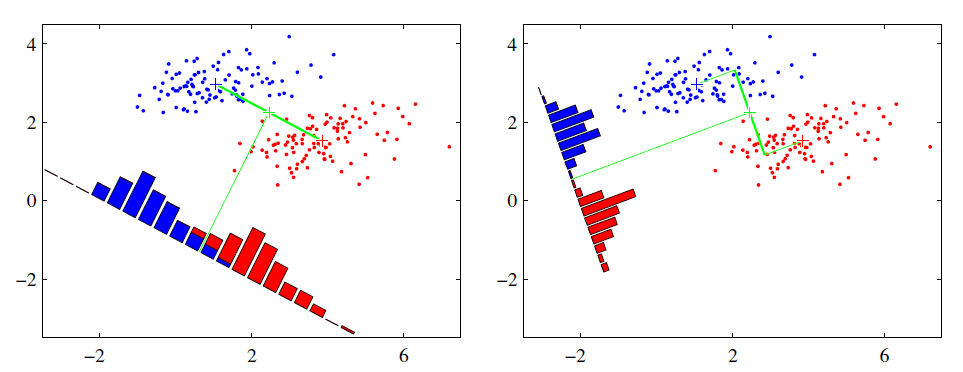
\includegraphics[width=0.55\textwidth]{lda-bi}
  \caption{二类LDA转换效果图 \label{fig:lda-bi}}
\end{figure}

假定数据集$D=\{(x_1, y_1), (x_2, y_2), ..., (x_m, y_m)\}$,其中$x_i \in R^{n}$,$y_i \in \{0, 1\}$。我们定义$N_j (j=0,1)$为第$j$类样本的个数,$X_j (j=0,1)$为第$j$类样本的合集,$\mu_j (i=0,1)$为第$j$类样本的均值向量,$\Sigma_j (j=0,1)$为第$j$类样本缺少分母部分的协方差矩阵。那么$\mu_j$和$\Sigma_j$的表达式分别如公式\ref{eqn:lda-mean}和公式\ref{eqn:lda-var}所示。
\begin{align}
\mu_j &= \frac{1}{N_j} \sum_{x\in{j}} x  \label{eqn:lda-mean}\\
\Sigma_j &= \sum_{x\in{j}} (x-\mu_{j})(x-\mu_{j})^{T} \label{eqn:lda-var}
\end{align}

由于只有两类数据,所以只需要将这些数据投影到一条直线上就可以,假设投影向量为$w$,则对任意一个样本,其在直线上的投影为$w^{T}x$,类别中心的投影分别为$w^{T}\mu_{0}$和$w^{T}\mu_{1}$,LDA要求不同类别之间的类别中心尽可能的远,所以需要最大化$\parallel w^{T}\mu_{0} - w^{T}\mu_{1} \parallel_{2}^{2}$,同时我们还希望同一类别尽可能接近,也就是样本投影之后的协方差尽可能的小,投影后的协方差如公式\ref{eqn:shadow-var}。
\begin{align}
\label{eqn:shadow-var}
\begin{split}
\Sigma_{j}^{'} &= \sum_{x\in{j}} (w^{T}x-w^{T}\mu_{j})(w^{T}x-w^{T}\mu_{j})^{T} \\
               &= \sum_{x\in{j}} w^{T}(x-\mu_{j})(x-\mu_{j})^{T}w \\
               &= w^{T}\Sigma_{j} w
\end{split}
\end{align}
所以我们希望最小化 $w^{T}\Sigma_{0} w + w^{T}\Sigma_{1} w$,由此我们可以得到需要优化的目标函数,如公式\ref{eqn:lda-obj-bi}。
\begin{align}
\label{eqn:lda-obj-bi}
\begin{split}
\arg\mathop{\max}_{w} J(w) &= \arg\mathop{\max}_{w}  \frac{\parallel w^{T}\mu_{0} - w^{T}\mu_{1} \parallel_{2}^{2}}{w^{T}\Sigma_{0} w + w^{T}\Sigma_{1} w} \\
                           &= \arg\mathop{\max}_{w}  \frac{w^{T} (\mu_{0} - \mu_{1}) (\mu_{0} - \mu_{1})^{T}w }{w^{T}(\Sigma_{0} + \Sigma_{1}) w} \
\end{split}
\end{align}

类内散度矩阵$S_w$和类间散度矩阵$S_b$分别定义为公式\ref{eqn:intra-matrix}和公式\ref{eqn:inter-matrix}。
\begin{align}
S_w &= \Sigma_{0} + \Sigma_{1} \label{eqn:intra-matrix}\\
S_b &= (\mu_{0} - \mu_{1}) (\mu_{0} - \mu_{1})^{T}  \label{eqn:inter-matrix}
\end{align}

所以目标函数就变成了:
\begin{align}
\label{eqn:lda-obj-bi-rui}
\arg\mathop{\max}_{w} J(w)  &= \arg\mathop{\max}_{w} \frac{w^{T}S_{b}w}{w^{T}S_{w}w} 
\end{align}

也就是求解出$w$使得$J(w)$最大。根据\ref{sec:rayleigh-quotient}中的介绍,我们可以通过计算矩阵$S_{w}^{-1}S_{b}$的特征值和特征向量得到对应的$w$,即求解公式\ref{eqn:lda-di-solve}。$J(w)$的最大值为$S_{w}^{-1}S_{b}$的最大特征值,最小值为$S_{w}^{-1}S_{b}$的最小特征值,而$S_w$和$S_b$均可由原始数据求解得出,因此很容易就可以求解出$J(w)$的最大值。
\begin{align}
\label{eqn:lda-di-solve}
S_{w}^{-1}S_{b}w = \lambda{w}
\end{align}

接下来我们分析下多类LDA的原理。

假定数据集$D=\{(x_1, y_1), (x_2, y_2), ..., (x_m, y_m)\}$,其中$x_i \in R^{n}$,$y_i \in \{C_1, C_2, ..., C_k\}$。我们定义$N_j (j=0,1,...,k)$为第$j$类样本的个数,$X_j (j=0,1,...,k)$为第$j$类样本的合集,$\mu_j (i=0,1,...,k)$为第$j$类样本的均值向量,$\Sigma_j (j=0,1,...,k)$为第$j$类样本缺少分母部分的协方差矩阵。此时是多类分类,因此投影后的空间不再是一条直线,而是一个超平面。假设投影后的低维空间维度为$d$,对应的基向量为$(w_1, w_2,..., w_d)$,基向量组成的矩阵为$W\in{R^{n*d}}$。

此时类内的散度矩阵$S_W$仍旧存在,如公式\ref{eqn:intra-multi}。
\begin{align}
\label{eqn:intra-multi}
S_W = \sum_{j=1}^{k} \Sigma_{j} 
\end{align}

但是类间的散度矩阵就有所不同了。此时用每个类别的均值到全局均值的距离来衡量类间距如图\ref{fig:lda-mul}。
\begin{figure}[htbp]
  \centering
  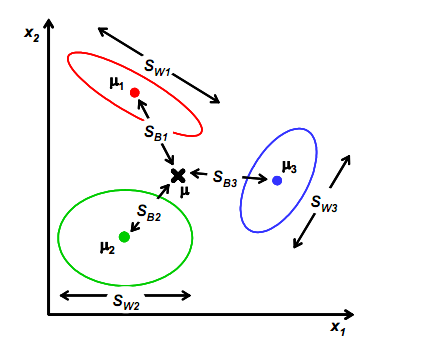
\includegraphics[width=0.55\textwidth]{lda-mul}
  \caption{多类LDA的类间散度矩阵示意图 \label{fig:lda-mul}}
\end{figure}

其定义为公式\ref{eqn:inter-multi}。
\begin{align}
\label{eqn:inter-multi}
S_B = \sum_{j=1}^{k} N_j (\mu_{j} - \mu)(\mu_{j} -\mu)^{T}
\end{align}
其中:
\begin{align}
\mu     &= \frac{1}{m}\sum_{i=1}^{m} x_{i} \\
\mu_{j} &= \frac{1}{N_{j}}\sum_{x_{j}\in{C_{j}}} x_{j}
\end{align}

同样此时的优化目标为公式\ref{eqn:lda-obj-multi}。
\begin{align}
\label{eqn:lda-obj-multi}
\arg\mathop{\max}_{W} J(W)  &= \arg\mathop{\max}_{W} \frac{W^{T}S_{B}W}{W^{T}S_{W}W} 
\end{align}

此时目标函数求解转换成了公式\ref{eqn:lda-mul-solve}:
\begin{align}
\label{eqn:lda-mul-solve}
S_{W}^{-1}S_{B}W = \lambda{W}
\end{align}

以上,可以总结出多类LDA的求解步骤:
\begin{enumerate}
  \item 计算每个类别的均值向量和方差,以及全局均值向量;
  \item 根据均值向量和方差,计算$S_w$和$S_B$;
  \item 对$S_{W}^{-1}S_{B}W = \lambda{W}$进行求解,求出$S_{W}^{-1}S_{B}$的特征值和特征向量;
  \item 对特征向量进行排序,设定低维空间的维度$d$,选取前$d$个特征值和特征向量,特征向量组合成投影矩阵$W$;
  \item 通过投影矩阵计算出投影后的输入数据$x_{i}^{'}=W^{T}x_{i}$;
  \item 得到输出的新数据集:$\{(x_{1}^{'}, y_1), (x_{2}^{'}, y_2), ..., (x_{m}^{'}, y_m)\}$。
\end{enumerate}

%------------------------------------------------------------------------------
%                                       MLLT
%------------------------------------------------------------------------------
\section{最大似然线性变换}
最大似然线性变换(Maximum Likelihood Linear Transform)

在HMM系统中,协方差矩阵的选择可以是对角阵,分块对角阵或者全矩阵。相对于对角阵来说,全矩阵的优势在于对特征向量元素之间关系的建模,劣势在于参数量巨大。

%------------------------------------------------------------------------------
%                                       Beta
%------------------------------------------------------------------------------
\section{Beta分布}
  
%------------------------------------------------------------------------------
%                                   MLE vs MAP
%------------------------------------------------------------------------------
\section{MLE和MAP}

\href{https://wiseodd.github.io/techblog/2017/01/01/mle-vs-map/}{MLE vs MAP}

